% Beamer Presentation Template
% Version adjusted as per user's specifications

\documentclass[
    11pt,           % Default font size
    % t,             % Align vertically to the top
    %aspectratio=169 % Uncomment for 16:9 aspect ratio
]{beamer}

% Path for images
\graphicspath{{img/}}

% Additional packages
\usepackage[alf]{abntex2cite} % ABNT citations
\usepackage{booktabs}         % Enhanced table lines
\usepackage{palatino}         % Palatino font
\usepackage[default]{opensans}% Open Sans font
\usepackage{subcaption}
%----------------------------------------------------------------------------------------
%   PACKAGES AND CONFIGURATIONS FOR CODE
%----------------------------------------------------------------------------------------
% Necessary packages for code formatting
\usepackage[utf8]{inputenc}
\usepackage{listings}
\usepackage{xcolor}

% Colors for syntax highlighting (VSCode Light Theme)
\definecolor{vscBackground}{RGB}{255,255,255}    % White background
\definecolor{vscKeyword}{RGB}{175,0,219}         % Purple for keywords
\definecolor{vscString}{RGB}{163,21,21}          % Red for strings
\definecolor{vscComment}{RGB}{0,128,0}           % Green for comments
\definecolor{vscFunction}{RGB}{121,94,38}        % Brown for functions
\definecolor{vscNumber}{RGB}{9,134,88}           % Dark green for numbers
\definecolor{vscOperator}{RGB}{175,0,219}        % Purple for operators
\definecolor{vscText}{RGB}{0,0,0}                % Black text
\definecolor{vscLineNr}{RGB}{128,128,128}        % Gray for line numbers

% General listings configuration for UTF-8
\lstset{
    inputencoding=utf8,
    extendedchars=true,
    literate=%
        {á}{{\'a}}1 {é}{{\'e}}1 {í}{{\'i}}1 {ó}{{\'o}}1 {ú}{{\'u}}1
        {Á}{{\'A}}1 {É}{{\'E}}1 {Í}{{\'I}}1 {Ó}{{\'O}}1 {Ú}{{\'U}}1
        {à}{{\`a}}1 {è}{{\`e}}1 {ì}{{\`i}}1 {ò}{{\`o}}1 {ù}{{\`u}}1
        {À}{{\`A}}1 {È}{{\`E}}1 {Ì}{{\`I}}1 {Ò}{{\`O}}1 {Ù}{{\`U}}1
        {ã}{{\~a}}1 {õ}{{\~o}}1 {Ã}{{\~A}}1 {Õ}{{\~O}}1
        {â}{{\^a}}1 {ê}{{\^e}}1 {î}{{\^i}}1 {ô}{{\^o}}1 {û}{{\^u}}1
        {Â}{{\^A}}1 {Ê}{{\^E}}1 {Î}{{\^I}}1 {Ô}{{\^O}}1 {Û}{{\^U}}1
        {ç}{{\c c}}1 {Ç}{{\c C}}1
        {€}{{\EUR}}1 {£}{{\pounds}}1
}

% Base configuration common to all languages
\lstdefinestyle{baseStyle}{
    backgroundcolor=\color{vscBackground},
    basicstyle=\ttfamily\small\color{vscText},
    breakatwhitespace=false,
    breaklines=true,
    captionpos=b,
    keepspaces=true,
    numbers=left,
    numbersep=5pt,
    showspaces=false,
    showstringspaces=false,
    showtabs=false,
    tabsize=4,
    frame=single,
    framerule=0.8pt,
    rulecolor=\color{gray!20},
    numberstyle=\tiny\color{vscLineNr},
    keywordstyle=\color{vscKeyword},
    commentstyle=\color{vscComment}\itshape,
    stringstyle=\color{vscString},
    emphstyle=\color{vscFunction},
    columns=flexible,
    basewidth={0.5em,0.45em},
    inputencoding=utf8,
    extendedchars=true
}

%----------------------------------------------------------------------------------------
% Python
%----------------------------------------------------------------------------------------
\lstdefinestyle{pythonStyle}{
    style=baseStyle,
    language=Python,
    morekeywords={self,None,True,False,import,from,as,def,class,return,yield,
                  for,while,if,else,elif,try,except,finally,with,lambda,
                  async,await,break,continue,global,nonlocal,pass,raise},
    morekeywords=[2]{print,len,range,type,int,str,float,list,dict,set,
                     tuple,max,min,sum,sorted,enumerate,zip,map,filter,
                     any,all,abs,round,pow,divmod},
    keywordstyle=[2]\color{vscFunction},
    sensitive=true
}

\lstnewenvironment{python}[1][]{\lstset{style=pythonStyle, #1}}{}
\newcommand{\pyinline}[1]{\lstinline[style=pythonStyle]!#1!}
\newcommand{\inputpython}[2][]{\lstinputlisting[style=pythonStyle,#1]{#2}}

%----------------------------------------------------------------------------------------
% C Language
%----------------------------------------------------------------------------------------
\lstdefinestyle{cStyle}{
    style=baseStyle,
    language=C,
    morekeywords={include,define,void,int,char,float,double,long,unsigned,
                  struct,union,enum,typedef,const,static,extern,register,
                  auto,volatile,sizeof,return,if,else,for,while,do,switch,
                  case,break,continue,default,goto},
    morekeywords=[2]{printf,scanf,malloc,free,calloc,realloc,fopen,fclose,
                     fprintf,fscanf,strcpy,strlen,strcat},
    keywordstyle=[2]\color{vscFunction},
    sensitive=true
}

\lstnewenvironment{clang}[1][]{\lstset{style=cStyle, #1}}{}
\newcommand{\clinline}[1]{\lstinline[style=cStyle]!#1!}
\newcommand{\inputclang}[2][]{\lstinputlisting[style=cStyle,#1]{#2}}

%----------------------------------------------------------------------------------------
% C++
%----------------------------------------------------------------------------------------
\lstdefinestyle{cppStyle}{
    style=baseStyle,
    language=C++,
    morekeywords={class,private,protected,public,template,typename,namespace,
                  using,new,delete,this,friend,virtual,override,final,explicit,
                  mutable,constexpr,nullptr,noexcept,static_cast,dynamic_cast,
                  const_cast},
    morekeywords=[2]{cout,cin,endl,vector,string,map,set,queue,stack,pair,
                     begin,end,push_back,pop_back,emplace_back,size,empty},
    keywordstyle=[2]\color{vscFunction},
    sensitive=true
}

\lstnewenvironment{cpp}[1][]{\lstset{style=cppStyle, #1}}{}
\newcommand{\cppinline}[1]{\lstinline[style=cppStyle]!#1!}
\newcommand{\inputcpp}[2][]{\lstinputlisting[style=cppStyle,#1]{#2}}

%----------------------------------------------------------------------------------------
% R Language
%----------------------------------------------------------------------------------------
\lstdefinestyle{rStyle}{
    style=baseStyle,
    language=R,
    morekeywords={if,else,repeat,while,function,for,in,next,break,TRUE,FALSE,
                  NULL,Inf,NaN,NA,NA_integer_,NA_real_,NA_complex_,NA_character_},
    morekeywords=[2]{library,require,attach,detach,source,setwd,options,
                     data.frame,read.csv,write.csv,list,matrix,array},
    keywordstyle=[2]\color{vscFunction},
    sensitive=true
}

\lstnewenvironment{rlang}[1][]{\lstset{style=rStyle, #1}}{}
\newcommand{\rlinline}[1]{\lstinline[style=rStyle]!#1!}
\newcommand{\inputrlang}[2][]{\lstinputlisting[style=rStyle,#1]{#2}}

%----------------------------------------------------------------------------------------
% Java
%----------------------------------------------------------------------------------------
\lstdefinestyle{javaStyle}{
    style=baseStyle,
    language=Java,
    morekeywords={abstract,assert,boolean,break,byte,case,catch,char,class,
                  const,continue,default,do,double,else,enum,extends,final,
                  finally,float,for,if,implements,import,instanceof,int,
                  interface,long,native,new,package,private,protected,public,
                  return,short,static,strictfp,super,switch,synchronized,this,
                  throw,throws,transient,try,void,volatile,while},
    morekeywords=[2]{String,System,out,println,printStackTrace,ArrayList,
                     HashMap,Arrays,List,Map,Set,Exception,RuntimeException},
    keywordstyle=[2]\color{vscFunction},
    sensitive=true
}

\lstnewenvironment{java}[1][]{\lstset{style=javaStyle, #1}}{}
\newcommand{\javainline}[1]{\lstinline[style=javaStyle]!#1!}
\newcommand{\inputjava}[2][]{\lstinputlisting[style=javaStyle,#1]{#2}}
     % Code formatting
\usepackage{tikz}
\usepackage{circuitikz}
\usetikzlibrary{arrows, shapes, shapes.geometric, positioning, matrix, patterns, arrows.meta, calc, shadows}
\tikzstyle{block} = [rectangle, draw, fill=blue!20, text width=3cm, text centered, rounded corners, minimum height=1cm]
\tikzstyle{line} = [draw, -latex', thick]
% In main.tex preamble
\usepackage{pgf-pie}      % For \pie command
\usepackage{pgfplots}     % For \begin{axis} environment
\pgfplotsset{compat=1.17} % Set compatibility level for pgfplots
\usepackage{hyperref}
\usepackage{multicol}
\usepackage{xcolor}

\usepackage{float}
\usepackage{opensans}

% Packages for graphics and charts
\usepackage{graphicx}
\usepackage{multirow}
\usepackage{caption}
\usepackage{color}
\usepackage{adjustbox} % For adjusting table sizes if needed

% nafees' animation 
\tikzset{
  invisible/.style={opacity=0},
  visible on/.style={alt={#1{}{invisible}}},
  alt/.code args={<#1>#2#3}{%
    \alt<#1>{\pgfkeysalso{#2}}{\pgfkeysalso{#3}} % \pgfkeysalso doesn't change the path
  },
}
\usepackage{tcolorbox}  % Provides tcbitemize and advanced box formatting
\usepackage{fontawesome5}  % For the \faTools icon
% \usepackage{pgfplots} % For creating plots
% \pgfplotsset{compat=1.18}
%nafees ends


% nafees' animation (25-32)
\tikzset{
  invisible/.style={opacity=0},
  visible on/.style={alt={#1{}{invisible}}},
  alt/.code args={<#1>#2#3}{%
    \alt<#1>{\pgfkeysalso{#2}}{\pgfkeysalso{#3}} % \pgfkeysalso doesn't change the path
  },
}

\usepackage{array}

%----------------------------------------------------------------------------------------
%   LAYOUT AND COLOR SELECTION
%----------------------------------------------------------------------------------------

\usetheme{Boadilla} % Layout theme

% Define custom colors
\definecolor{primaryColor}{RGB}{20,45,105}     % Primary color
\definecolor{secondaryColor}{RGB}{0,100,160}   % Secondary color
\definecolor{footerBottomColor}{RGB}{15,75,130} % Footer bottom color (adjusted for visual appeal)
% Define colors for correct and incorrect labels
\definecolor{mygreen}{RGB}{34,139,34}
\definecolor{myred}{RGB}{178,34,34}
\definecolor{myblue}{RGB}{0,0,255}
\definecolor{myorange}{RGB}{255,165,0}
\definecolor{blue}{RGB}{31,119,180}
\definecolor{red}{RGB}{214,39,40}
\definecolor{green}{RGB}{44,160,44}
\definecolor{orange}{RGB}{255,127,14}
\definecolor{goldenrod}{rgb}{0.85, 0.65, 0.13} % RGB values for goldenrod


% Apply colors to the theme
\setbeamercolor{structure}{fg=primaryColor}
\setbeamercolor{palette primary}{bg=primaryColor, fg=white}
\setbeamercolor{palette secondary}{bg=secondaryColor, fg=white}
\setbeamercolor{title}{bg=primaryColor, fg=white} % Main title color

% Colors in the header
\setbeamercolor{headline}{bg=secondaryColor, fg=white}
\setbeamercolor{section in head/foot}{bg=primaryColor, fg=white}
\setbeamercolor{subsection in head/foot}{bg=secondaryColor, fg=white}

% Footer color configurations
\setbeamercolor{author in head/foot}{bg=primaryColor, fg=white} % Left partition
\setbeamercolor{institute in head/foot}{bg=secondaryColor, fg=white} % Right partition
\setbeamercolor{title in head/foot}{bg=footerBottomColor, fg=white} % Bottom line

% Inner and outer themes
\useinnertheme{circles}   % Inner theme
\useoutertheme{miniframes} % Outer theme

%\setbeamertemplate{navigation symbols}{} % Remove navigation symbols (Commented out to enable them)

% TikZ styles for flowcharts
\tikzstyle{startstop} = [rectangle, rounded corners, minimum width=2.5cm, minimum height=1cm, text centered, draw=black, fill=primaryColor!20]
\tikzstyle{process} = [rectangle, minimum width=2.5cm, minimum height=1cm, text centered, draw=black, fill=secondaryColor!20]
\tikzstyle{arrow} = [thick,->,>=stealth]

%------------------
%   PRESENTATION INFORMATION
%------------------

% \title[ChatGPT Incorrectness Detection in Software Reviews]{ChatGPT Incorrectness Detection in Software Reviews}
% \author[Nafis \textbar{} Nafees \textbar{} Raihan]{
%     \textbf{Nafis Nahian} {\scriptsize \texttt{(2105007)}} \\ 
%     \textbf{Sk. Ashrafuzzaman Nafees} {\scriptsize \texttt{(2105008)}} \\ 
%     \textbf{Abrar Zahin Raihan} {\scriptsize \texttt{(2105009)}}
% }
% \institute[Bangladesh University of Engineering and Technology]{\textbf{Bangladesh University of Engineering and Technology} \\ \vspace{0.5em} \tiny{Department of Computer Science and Engineering}}
% \date[Year]{\textbf{\today}}

\title[ChatGPT Incorrectness Detection in Software Reviews]{ChatGPT Incorrectness Detection in Software Reviews}

\author[Nafis \textbar{} Nafees \textbar{} Raihan]{
    \noindent
\begin{tabular}{p{0.45\linewidth}|>{\raggedleft\arraybackslash}p{0.45\linewidth}}
    \textbf{\Large Authors} & \textbf{\Large Presented by} \\
    \small Minaoar Hossain Tanzil & \small Nafis Nahian {\tiny \texttt{(2105007)}} \\
    \small Junaed Younus Khan & \small Nafees Ashraf {\tiny \texttt{(2105008)}} \\
    \small Gias Uddin & \small Abrar Zahin Raihan {\tiny \texttt{(2105009)}} \\
\end{tabular}
}

\institute[Bangladesh University of Engineering and Technology]{\textbf{Bangladesh University of Engineering and Technology} \\ \vspace{0.5em} \tiny{Department of Computer Science and Engineering}}
\date[Year]{\textbf{\today}}


\institute[Bangladesh University of Engineering and Technology]{\textbf{Bangladesh University of Engineering and Technology} \\ \vspace{0.5em} \tiny{Department of Computer Science and Engineering}}
\date[Year]{\textbf{\today}}


%------------------
%   ADD OUTLINE BEFORE EACH SECTION
%------------------

\AtBeginSection[]{
  \begin{frame}
    \frametitle{Outline}
    \tableofcontents[currentsection]
  \end{frame}
}

%------------------
%   CUSTOM FOOTER
%------------------

\setbeamertemplate{footline}{
  \leavevmode%
  \vbox{%
    % First line with partitions
    \hbox{%
      % Left partition (Your Name)
      \begin{beamercolorbox}[wd=.475\paperwidth,ht=2.25ex,dp=1ex,leftskip=0.3cm,rightskip=0cm]{author in head/foot}%
        \usebeamerfont{author in head/foot}%
        \hspace*{0pt}\insertshortauthor%
      \end{beamercolorbox}%
      % Vertical separator
      \begin{beamercolorbox}[wd=0pt,ht=2.25ex,dp=1ex]{separator}%
        \hspace*{-0.2pt}%
        \color{white}\vrule width 0.5pt%
      \end{beamercolorbox}%
      % Right partition (Your Institution)
      \begin{beamercolorbox}[wd=.525\paperwidth,ht=2.25ex,dp=1ex,leftskip=0cm,rightskip=0.3cm]{institute in head/foot}%
        \usebeamerfont{institute in head/foot}%
        \hfill\insertshortinstitute%
      \end{beamercolorbox}%
    }%
    % Second line without partitions
    \hbox{%
      \begin{beamercolorbox}[wd=\paperwidth,ht=2.25ex,dp=1ex,leftskip=0.3cm,rightskip=0.3cm]{title in head/foot}%
        \usebeamerfont{title in head/foot}%
        \hspace*{0pt}\insertshorttitle%
        \hfill%
        \insertframenumber{}/\inserttotalframenumber%
      \end{beamercolorbox}%
    }%
  }%
}



%------------------

\begin{document}

%------------------
%   TITLE SLIDE
%------------------

\begin{frame}
    % \begin{figure}
    %     \includegraphics[width=0.3\linewidth]{img/your_logo.png} % Add your logo here
    % \end{figure}
    \titlepage % Display the title slide
\end{frame}

%------------------
%   TABLE OF CONTENTS SLIDE
%------------------

\begin{frame}
    \frametitle{Presentation Outline} % Slide title
    \tableofcontents % Display the table of contents
\end{frame}

%------------------
%   PRESENTATION BODY SECTIONS
%------------------

\section{Introduction}



\begin{frame}{Background}
    \begin{columns}
        % Column 1: Text
        \column{0.6\textwidth}
        \textbf{\textit{Generative AI tools like ChatGPT are revolutionizing various domains, including software engineering. But can we trust their responses?}}
        
        % Column 2: Image
        \column{0.4\textwidth}
        
\includegraphics[width=\textwidth]{image2.jpg}
    \end{columns}
\end{frame}

%------------------------------------------------
\begin{frame}
    \frametitle{Background}
    \vspace{0.5cm}
    \textit{Developers are increasingly using ChatGPT for SE tasks like library selection}
    \vspace{0.5cm}
    \begin{figure}[!ht]
        \centering
        \resizebox{0.6\textwidth}{!}{% Adjusted the size to make it bigger
        \begin{circuitikz}
        \tikzstyle{every node}=[font=\Large]        
        \draw (10.75,11.5) rectangle (10.75,11.5);
        \draw [fill={rgb,255:red,209; green,240; blue,255}, rounded corners=7.2] (9.75,12.25) rectangle (14.5,11);
        \draw [fill={rgb,255:red,209; green,240; blue,255}, rounded corners=7.2] (9.5,9.5) rectangle (14.5,8.25);
        \draw [fill={rgb,255:red,209; green,240; blue,255}, rounded corners=6.0] (6,6.25) rectangle (9,5);
        \draw [fill={rgb,255:red,209; green,240; blue,255}, rounded corners=6.0] (10.75,6.25) rectangle (13.5,5);
        \draw [fill={rgb,255:red,209; green,240; blue,255}, rounded corners=6.0] (15.25,6.25) rectangle (18,5);
        \draw [short] (7.5,6.25) -- (7.5,7.25);
        \draw [short] (12,6.25) -- (12,7.25);
        \draw [short] (8.25,7.25) -- (16.75,7.25);
        \draw [short] (16.75,7.25) -- (16.75,6.25);
        \draw [short] (7.5,7.25) -- (8.25,7.25);
        \node at (12.15,11.6) {Driver Code};
        \node at (12,8.9) {Framework};
        \node at (7.5,5.5) {Library};
        \node at (12.15,5.5) {Library};
        \node at (16.65,5.5) {Library};
        \node [font=\small] at (12.25,10.25) {Code uses framework};
        \node [font=\small] at (12,7.5) {Framework contains library};
        \draw [short] (12,9.5) -- (12,10);
        \draw [->, >=Stealth] (12,10.5) -- (12,11);
        \draw [->, >=Stealth] (12,8) -- (12,8.25);
        \draw [short] (12,8) -- (12,7.75);
        \end{circuitikz}
        }%
        \label{meumeu}
    \end{figure}
\end{frame}
%------------------------------------------------
\begin{frame}
    \frametitle{Overview}
    \begin{figure}[!ht]
        \centering
        \resizebox{0.55\textwidth}{!}{%
        \begin{circuitikz}
        \tikzstyle{every node}=[font=\LARGE]
        \node [font=\LARGE] at (2.75,10.25) {};
        \draw (6,11.75) to[short] (6,4.25);
        \draw [->, >=Stealth] (6,4.25) -- (8.25,4.25);
        \node [font=\Large] at (10.75,12.75) {\underline{Phase 1}};
        \node [font=\large] at (10.75,12) {Survey to learn };
        \node [font=\large] at (10.75,11.5) {preferences and };
        \draw  (10.75,12) circle (2.25cm);
        \node [font=\large, rotate around={-360:(0,0)}] at (10.75,11) {concerns};
        \draw [->, >=Stealth] (6,11.75) -- (8.5,11.75);
        \draw [->, >=Stealth] (4.75,8) -- (6,8);
        \node [font=\Large] at (10.75,5.25) {\underline{Phase 2}};
        \node [font=\large] at (10.75,4.5) {Developed a tool};
        \node [font=\large] at (10.85,3.5) {ChatGPT Incorrectness};
        \node [font=\large] at (10.75,4) {called CID aka};
        \node [font=\large, rotate around={-360:(0,0)}] at (10.75,3) {Detector};
        \draw  (10.75,4.25) circle (2.5cm);
        \draw [ fill={rgb,255:red,204; green,245; blue,255} , rounded corners = 11.4, rotate around={-360:(2.75, 8)}] (0.75,8.75) rectangle (4.75,7.25);
        \node [font=\LARGE] at (2.75,8) {Research};
        \end{circuitikz}
        }%
        \label{meumeu}
        \end{figure}
\end{frame}

%------------------------------------------------
\setbeamercovered{transparent}
\begin{frame}
    \frametitle{Overview}
    \begin{itemize}
        \item Focus on software library selection as a case study. \pause
        \item Need for understanding how developers use ChatGPT and their concerns. \pause
        \item Desire for automated tools to detect incorrectness in ChatGPT's outputs.
    \end{itemize}
\end{frame}

%------------------------------------------------

\section{Survey of Software Developers}

%------------------------------------------------

\begin{frame}
    \frametitle{Survey Overview}
    \begin{itemize}
        \item Conducted a survey with 135 SE practitioners.
        \item Aimed to answer three Research Questions (RQs):
        \begin{itemize}
            \item \textbf{RQ1:} Why do software developers use ChatGPT?
            \item \textbf{RQ2:} How much do developers rely on ChatGPT responses?
            \item \textbf{RQ3:} How do developers verify ChatGPT responses?
        \end{itemize}
    \end{itemize}
\end{frame}

%-----------------------------

\begin{frame}
    \frametitle{Participant Demographics (Current Profession)}
    \vspace{0.5cm}
    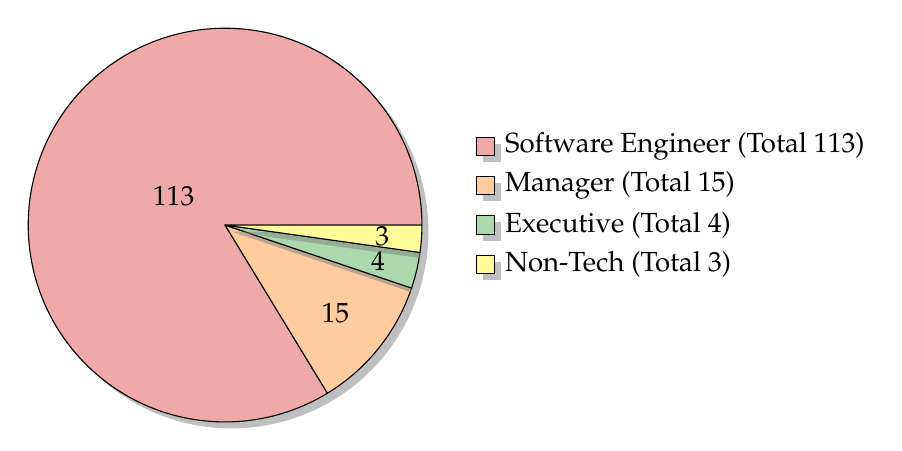
\begin{tikzpicture}
        \pie[
            text=legend,
            radius=2.5,
            color={red!40, orange!40, green!40, yellow!40},
            before number=,
            after number=,
            style=drop shadow,
            sum=135
        ]{
            113/Software Engineer (Total 113),
            15/Manager (Total 15),
            4/Executive (Total 4),
            3/Non-Tech (Total 3)
        }
        \end{tikzpicture}
        
        \vspace{1em} % Add some vertical spacing
        \begin{center}
            \textbf{Total Participants = 135}
        \end{center}
\end{frame}


%------------------------------------------------

\begin{frame}
    \frametitle{Participant Demographics (Years of Experience)}
    \vspace{0.5cm}
    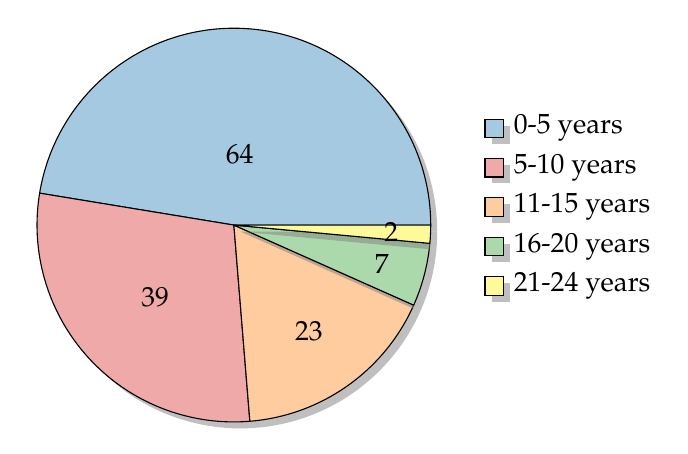
\begin{tikzpicture}
        \pie[
            text=legend,
            radius=2.5,
            color={blue!40, red!40, orange!40, green!40, yellow!40},
            before number=,
            after number=,
            style=drop shadow,
            sum=135
        ]{
            64/0-5 years,
            39/5-10 years,
            23/11-15 years,
            7/16-20 years,
            2/21-24 years
        }
        \end{tikzpicture}
        
        \vspace{1em} % Add some vertical spacing
        \begin{center}
            \textbf{Total Participants = 135}
        \end{center}
\end{frame}



%--------------------------------------------

\begin{frame}
    \frametitle{Survey Questions}
    {\scriptsize
        \begin{table}
\caption{Survey questions and their mapping to
the Research Questions. Here, C/O=Close/Open-ended question, G/S=Generic/Scenario-based question. For scenario-based questions, we used library selection as a case-study.}
\label{tab:survey_questions_on_chatgpt}
\resizebox{\linewidth}{!}{
\begin{tabular}{c p{9cm} c c c}
\hline
\textbf{Q\#} & \textbf{Questions} & \textbf{O/C} & \textbf{G/S} & \textbf{RQ} \\ \hline
1 & Did you use ChatGPT? & C & G & 1.1 \\
2 & In general, which of the cases you used it for? & C & G & 1.1 \\
3 & As a software professional, how did you or can you use it? & C & G & 1.1 \\
4 & How would you describe your experience with using it so far? & C & G & 1.1 \\
5 & How much do you rely on the content/response of ChatGPT? & C & G & 1.2 \\
6 & Have you considered using ChatGPT to select or compare software libraries? 
    Please share the pros and cons. & O & S & 1.2 \\
7 & How much would you rely on ChatGPT's response for the given library selection query? & C & S & 1.3 \\
8 & Would you rely on the ChatGPT's response after further inquiry? & C & S & 1.3 \\
9 & Do you think the opinion from ChatGPT is correct? & C & S & 1.3 \\
10 & What can be the ways to improve the reliability of ChatGPT responses? & C & G & 1.3 \\ \hline
\end{tabular}
}
\vspace{-4mm}
\end{table}

    }
\end{frame}


%------------------------------------------------
\begin{frame}
    \frametitle{Reasons to use ChatGPT (RQ1)}
    \textbf{The answers to the following questions help us to find the answer to Why developers used ChatGPT}
    \vspace{1cm}
    \begin{enumerate}
        \item Did you use ChatGPT?
        \item In general, which of the cases you used it for?
        \item As a software professional, how did you or can you use it? 
        \item How would you describe your experience with using it so far? 
    \end{enumerate}

\end{frame}

%--------------------------
\begin{frame}
    \frametitle{Reasons to use ChatGPT (RQ1)}
    \vspace{2em}
    \textbf{1. Did you use ChatGPT}
    \vspace{1cm}
    \begin{tikzpicture}
        \begin{axis}[
        xbar,
        xmin=0,
        xmax=100,
        width=0.8\linewidth,
        height=0.35\textheight,
        enlarge y limits=0.15,
        symbolic y coords={
        YES,NO
        },
        ytick=data,
            y tick label style={align=left, font=\footnotesize}, % Correct alignment
            nodes near coords,
            nodes near coords align={horizontal},
            axis lines*=left,
            y axis line style={opacity=0},
            x axis line style={opacity=0},
            tickwidth=0pt,
            enlarge x limits=0.02,
        ]
        \addplot[fill=red!80!white] coordinates {
        (98.52,YES)
        (1.48,NO)
        };
        \end{axis}
        \end{tikzpicture}
\end{frame}


%--------------------------

\begin{frame}
    \frametitle{Reasons to use ChatGPT (RQ1)}
    \vspace{1em}
    \textbf{2. In general, which of the cases you used it for?}
    \begin{tikzpicture}
        \begin{axis}[
            xbar,
            xmin=0,
            xmax=100,
            width=\linewidth,
            height=\textheight,
            bar width=6pt,
            enlarge y limits=0.15,
            symbolic y coords={
                Others,
                {Research for \\ Product Dev.},
                {Data Collection},
                Decision Making,
                Content Creation,
                {Learning \& \\ Knowledge Acq.},
                As a Search Engine,
                Just for Fun
            },
            ytick=data,
            y tick label style={align=left, font=\footnotesize},
            nodes near coords,
            nodes near coords align={horizontal},
            axis lines*=left,
            y axis line style={opacity=0},
            x axis line style={opacity=0},
            tickwidth=0pt,
            enlarge x limits=0.02,
        ]
        % Bars appear incrementally
        
        \only<1>{\addplot[fill=blue!80!white] coordinates {(42.22,Just for Fun)};}
        \only<2>{\addplot[fill=blue!80!white] coordinates {(42.22,Just for Fun) (79.26,As a Search Engine)};}
        \only<3>{\addplot[fill=blue!80!white] coordinates {(42.22,Just for Fun) (79.26,As a Search Engine) (61.48,{Learning \& \\ Knowledge Acq.})};}
        \only<4>{\addplot[fill=blue!80!white] coordinates {(42.22,Just for Fun) (79.26,As a Search Engine) (61.48,{Learning \& \\ Knowledge Acq.}) (46.67,Content Creation)};}
        \only<5>{\addplot[fill=blue!80!white] coordinates {(42.22,Just for Fun) (79.26,As a Search Engine) (61.48,{Learning \& \\ Knowledge Acq.}) (46.67,Content Creation) (48.15,Decision Making)};}
        \only<6>{\addplot[fill=blue!80!white] coordinates {(42.22,Just for Fun) (79.26,As a Search Engine) (61.48,{Learning \& \\ Knowledge Acq.}) (46.67,Content Creation) (48.15,Decision Making) (27.41,{Data Collection})};}
        \only<7>{\addplot[fill=blue!80!white] coordinates {(42.22,Just for Fun) (79.26,As a Search Engine) (61.48,{Learning \& \\ Knowledge Acq.}) (46.67,Content Creation) (48.15,Decision Making) (27.41,{Data Collection}) (28.15,{Research for \\ Product Dev.})};}
        \only<8>{\addplot[fill=blue!80!white] coordinates {(42.22,Just for Fun) (79.26,As a Search Engine) (61.48,{Learning \& \\ Knowledge Acq.}) (46.67,Content Creation) (48.15,Decision Making) (48.15,Decision Making) (27.41,{Data Collection}) (28.15,{Research for \\ Product Dev.}) (1.32,Others)};}
        \end{axis}
    \end{tikzpicture}
\end{frame}


%------------------------


\begin{frame}
    \frametitle{Reasons to use ChatGPT (RQ1)}
    \vspace{1em}
    \textbf{3.  As a software professional, how did you or can you use it?}
    \begin{tikzpicture}
        \begin{axis}[
            xbar,
            xmin=0,
            xmax=100,
            width=\linewidth,
            height=\textheight,
            bar width=6pt,
            enlarge y limits=0.15,
            symbolic y coords={
                {Code Generation \\ and Optimization},
                {Code Analysis \\ and review},
                {Solving \\ Support},
                {Alternative \\ Approaches},
                {Library \\ Selection},Others
            },
            ytick=data,
            y tick label style={align=left, font=\footnotesize},
            nodes near coords,
            nodes near coords align={horizontal},
            axis lines*=left,
            y axis line style={opacity=0},
            x axis line style={opacity=0},
            tickwidth=0pt,
            enlarge x limits=0.02,
        ]
        % Bars appear incrementally
        
        \only<1>{\addplot[fill=green!80!white] coordinates {(60,{Code Generation \\ and Optimization})};}
        \only<2>{\addplot[fill=green!80!white] coordinates {(60,{Code Generation \\ and Optimization}) (52.59,{Code Analysis \\ and review})};}
        \only<3>{\addplot[fill=green!80!white] coordinates {(60,{Code Generation \\ and Optimization}) (52.59,{Code Analysis \\ and review}) (86,{Solving \\ Support})};}
        \only<4>{\addplot[fill=green!80!white] coordinates {(60,{Code Generation \\ and Optimization}) (52.59,{Code Analysis \\ and review}) (86,{Solving \\ Support}) (73.33,{Alternative \\ Approaches})};}
        \only<5>{\addplot[fill=green!80!white] coordinates {(60,{Code Generation \\ and Optimization}) (52.59,{Code Analysis \\ and review}) (86,{Solving \\ Support}) (73.33,{Alternative \\ Approaches}) (46.67,{Library \\ Selection})};}
        \only<6>{\addplot[fill=green!80!white] coordinates {(60,{Code Generation \\ and Optimization}) (52.59,{Code Analysis \\ and review}) (86,{Solving \\ Support}) (73.33,{Alternative \\ Approaches}) (46.67,{Library \\ Selection}) (2,Others)};}
        \end{axis}
    \end{tikzpicture}
\end{frame}

%---------------------------

\begin{frame}
    \frametitle{Reasons to use ChatGPT (RQ1)}
    \vspace{1em}
    \textbf{4. How would you describe your experience with using it so far?}
    \begin{tikzpicture}
        \begin{axis}[
            xbar,
            xmin=0,
            xmax=100,
            width=\linewidth,
            height=0.7\textheight,
            bar width=6pt,
            enlarge y limits=0.15,
            symbolic y coords={
                Exciting,
                {Tech \\ Marvel},
                Unreliable,
                Over-hyped,
                Suspicious
            },
            ytick=data,
            y tick label style={align=left, font=\footnotesize},
            nodes near coords,
            nodes near coords align={horizontal},
            axis lines*=left,
            y axis line style={opacity=0},
            x axis line style={opacity=0},
            tickwidth=0pt,
            enlarge x limits=0.02,
        ]
        \addplot[fill=purple!80!white] coordinates {
            (68.15,Exciting)
            (42.22,{Tech \\ Marvel})
            (34,Unreliable)
            (19.26,Over-hyped)
            (9.63,Suspicious)
        };
        \end{axis}
    \end{tikzpicture}
\end{frame}

%----------------------------

\begin{frame}
    \frametitle{Summarizing Key Findings for RQ1}
    \begin{itemize}
        \item \textbf{Usage Purposes:}
        \begin{itemize}
            \item Code generation and optimization.
            \item Problem-solving support.
            \item Exploring alternative approaches.
            \item Library selection.
        \end{itemize}
        \item \textbf{Experience:}
        \begin{itemize}
            \item Excitement and recognition of technological advancement.
            \item Concerns about reliability and overhyped expectations.
        \end{itemize}
    \end{itemize}
\end{frame}



%------------------------------------------------


\begin{frame}
    \frametitle{Concerns About ChatGPT Responses (RQ2)}
    \textbf{We asked the following questions to the participants to find out how reliable ChatGPT is}
    \vspace{1cm}
    \begin{enumerate}
        \item How much do you rely on the content/response of ChatGPT?
        \item Have you considered using ChatGPT to select or compare software
        libraries? Please share the pros and cons?
    \end{enumerate}

\end{frame}

%----------------------------------------------
\begin{frame}
    \frametitle{Concerns About ChatGPT Responses (RQ2)}
    \textbf{1. How much do you rely on the content/response of ChatGPT?}
    \vspace{1cm}
    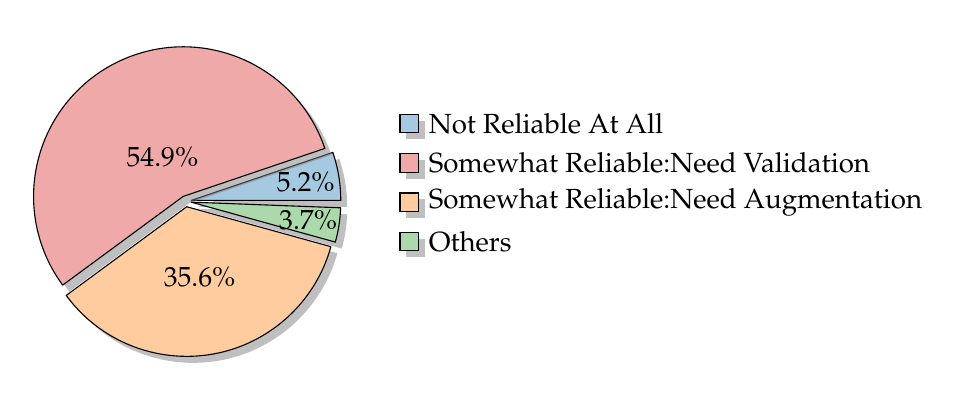
\begin{tikzpicture}
        \pie[
            text=legend,
            radius=1.9,
            color={blue!40, red!40, orange!40, green!40, yellow!40},
            before number=,
            after number={\%},
            style=drop shadow,
            explode=0.07
        ]{
            5.2/Not Reliable At All,
            54.9/Somewhat Reliable:Need Validation,
            35.6/Somewhat Reliable:Need Augmentation,
            3.7/Others
        }
        \end{tikzpicture}
\end{frame}

%------------------------------------------------

\begin{frame}
    \frametitle{Concerns About ChatGPT Responses (RQ2)}
    \vspace{1em}
    \textbf{2. Have you considered using ChatGPT to select or compare
    software libraries? Please share the pros and cons?}
    \vspace{0.5em}
    \begin{itemize}
        \item PROS :
        \begin{enumerate}
            \item Efficient Access to Information
            \item Initial Idea Generation
            \item Personalized Recommendations
            \item Time-Saving
        \end{enumerate}
        \vspace{0.5em}
        \item CONS :
        \begin{enumerate}
            \item Lack of Up-to-dateness
            \item Contextual Understanding Challenges
            \item Reliability Concerns
            \item Dependence on Prompt
            \item Not Sufficient for Decision-Making
            \item Bias of Training Data
        \end{enumerate}
        
    \end{itemize}
    
\end{frame}


%--------------------------------
\begin{frame}
    \frametitle{Pros and Cons for Library Selection (RQ2)}
    \vspace{0.5em}

    \begin{minipage}{\textwidth}
        \textbf{Pros : Total 45 responses}
        \centering
        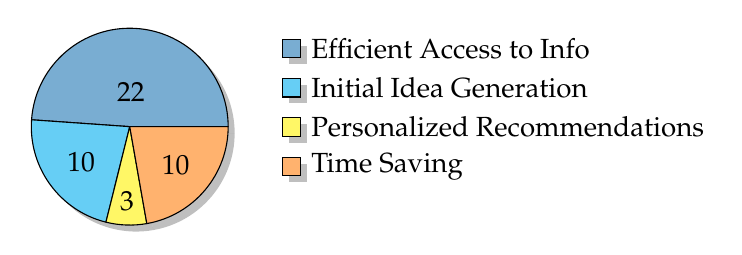
\begin{tikzpicture}
            \pie[text=legend, radius=1.25, sum=45, style=drop shadow]{
                22/Efficient Access to Info,
                10/Initial Idea Generation,
                3/Personalized Recommendations,
                10/Time Saving
            }
        \end{tikzpicture}
    \end{minipage}

    \vspace{1em} % Adds space between the pie charts

    \begin{minipage}{\textwidth}
        \textbf{Cons : Total 60 Responses}
        \centering
        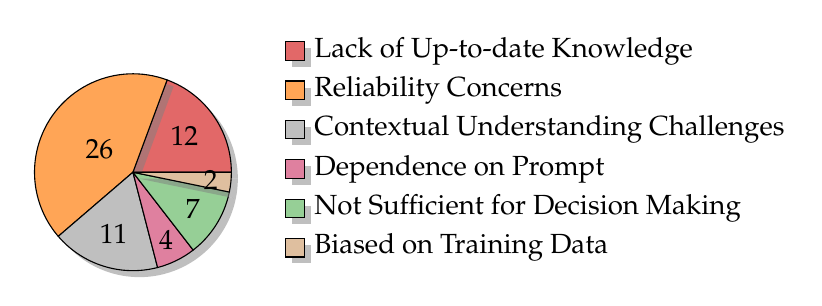
\begin{tikzpicture}
            \pie[text=legend, radius=1.25, color={red!70!white, orange!70!white, gray!50, purple!50, green!50, brown!50}, sum=62, style=drop shadow]{
                12/Lack of Up-to-date Knowledge,
                26/Reliability Concerns,
                11/Contextual Understanding Challenges,
                4/Dependence on Prompt,
                7/Not Sufficient for Decision Making,
                2/Biased on Training Data
            }
        \end{tikzpicture}
    \end{minipage}

\end{frame}

%-------------------------------------------------
\begin{frame}
    \frametitle{Key Findings for RQ2}
    \begin{itemize}
        \item \textbf{Reliability Concerns:}
        \begin{itemize}
            \item Only a small percentage fully trust ChatGPT responses.
            \item Majority consider the responses somewhat reliable but require validation.
        \end{itemize}
    \end{itemize}

      % Define colors within the frame
  \begin{tikzpicture}[scale=0.5, transform shape]
    % Local color definitions
    \definecolor{DeciderColor}{RGB}{102, 102, 238}    % Blue
    \definecolor{ChallengerColor}{RGB}{119, 209, 243}  % Green
    \definecolor{EnqColor}{RGB}{241, 230, 145}        % Orange
    \definecolor{MixedColor}{RGB}{244, 182, 114}     % Purple
    \definecolor{GreyColor}{RGB}{192, 192, 192}     % Grey for blurred slices

    % Overlay 1: Highlight Decider
    \only<1>{
        \pie[
      cloud,
      text=legend,
      scale font,
      radius=3, % Increased radius for more space
      % Optionally adjust font size
      color={
          DeciderColor,
          ChallengerColor,
          EnqColor,
          MixedColor
        },
      font=\scriptsize
    ]{
      34/Unreliaable,
      19.26/Over hyped,
      2.74/Fully Reliable, % Abbreviated label
      54/Somewhat Reliable
    }
    }
    \only<2>{
      \pie[
        cloud,
        text=legend,
        scale font,
        radius=3,
        color={
          DeciderColor,
          GreyColor,
          GreyColor,
          GreyColor
        },
        font=\scriptsize
      ]{
        34/Unreliaable,
        19.26/Over hyped,
        2.74/Fully Reliable, % Abbreviated label
        54/Somewhat Reliable
      }
    }

    % Overlay 2: Highlight Challenger
    \only<3>{
      \pie[
        cloud,
        text=legend,
        scale font,
        radius=3,
        color={
          GreyColor,
          ChallengerColor,
          GreyColor,
          GreyColor
        },
        font=\scriptsize
      ]{
        34/Unreliaable,
        19.26/Over hyped,
        2.74/Fully Reliable, % Abbreviated label
        54/Somewhat Reliable
      }
    }

    % Overlay 3: Highlight Enquirer
    \only<4>{
      \pie[
        cloud,
        text=legend,
        scale font,
        radius=3,
        color={
          GreyColor,
          GreyColor,
          EnqColor,
          GreyColor
        },
        font=\scriptsize
      ]{
        34/Unreliaable,
        19.26/Over hyped,
        2.74/Fully Reliable, % Abbreviated label
        54/Somewhat Reliable
      }
    }

    % Overlay 4: Highlight Mixed
    \only<5>{
      \pie[
        cloud,
        text=legend,
        scale font,
        radius=3,
        color={
          GreyColor,
          GreyColor,
          GreyColor,
          MixedColor
        },
        font=\scriptsize
      ]{
        34/Unreliaable,
        19.26/Over hyped,
        2.74/Fully Reliable, % Abbreviated label
        54/Somewhat Reliable
      }
    }
  \end{tikzpicture}
\end{frame}

%------------------------------------------------

%------------------------------------------------
\begin{frame}{Verification of ChatGPT Responses (RQ3)}
    Participants were presented with conversations with ChatGPT where it was asked
    \begin{itemize}
        \item Suggestions 
        \item More detail about a specific situation
        \item Reliability in SE real-world situations
    \end{itemize}
\end{frame}

\begin{frame}{Key Findings}
    \begin{center}
        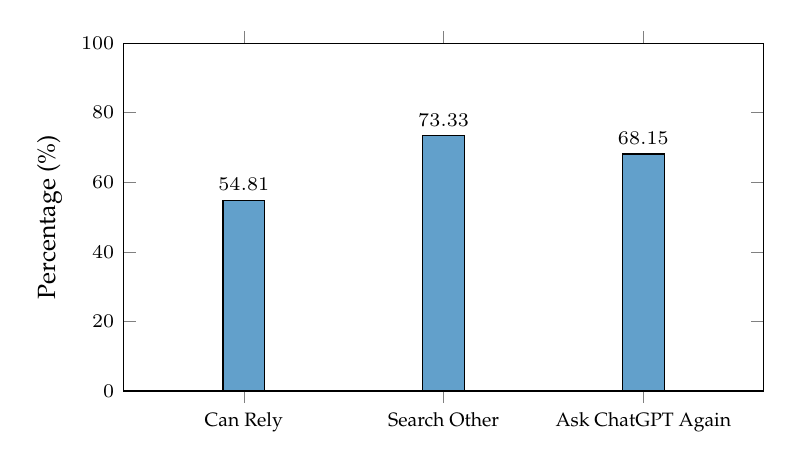
\begin{tikzpicture}
            \begin{axis}[
                ybar,
                bar width=15pt,
                width=0.8\textwidth,
                height=6cm,
                symbolic x coords={Can Rely, Search Other, Ask ChatGPT Again},
                xtick=data,
                xlabel={},
                ylabel={Percentage (\%)},
                ymin=0, ymax=100,
                nodes near coords,
                nodes near coords align={vertical},
                every node near coord/.append style={font=\scriptsize},
                enlarge x limits=0.3,
                ylabel style={font=\small},
                xlabel style={font=\small},
                ticklabel style={font=\scriptsize}
            ]
                % Data points
                \addplot[fill=blue!70] coordinates {
                    (Can Rely, 54.81)
                    (Search Other, 73.33)
                    (Ask ChatGPT Again, 68.15)
                };
            \end{axis}
        \end{tikzpicture}
    \end{center}
\end{frame}


%------------------------------------------------

\section{CID: ChatGPT Incorrectness Detector}

%------------------------------------------------

\begin{frame}
    \frametitle{Introducing CID}
    \begin{itemize}
        \item CID (ChatGPT Incorrectness Detector) tool
uses iterative prompting to capture ChatGPT’s inconsistency in a
similar fashion to an actual Crime Investigation Department (CID).
    \end{itemize}
\end{frame}

\begin{frame}{CID Tool Components}
    \begin{center}
    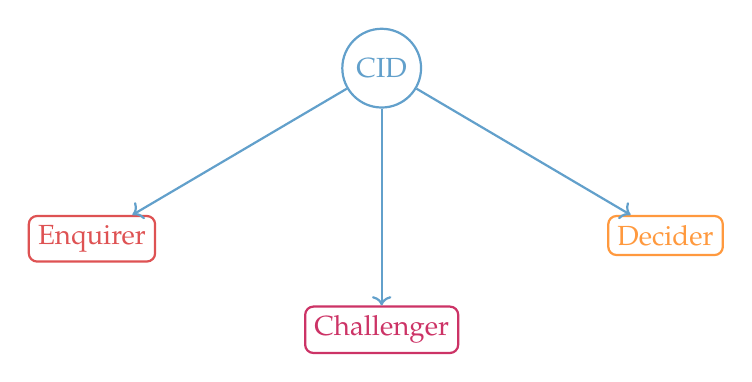
\begin{tikzpicture}
        % Main CID node
        \node[draw, circle, minimum size=1cm, thick, color=blue!70,visible on=<1->] (CID) at (7, 6.5) {CID};

        % Enquirer node
        \node[draw, rectangle, rounded corners=3pt, thick, color=red!80, below left=1.5cm and 2.5cm of CID,visible on=<2->] (Enquirer) {Enquirer};

        % Challenger node
        \node[draw, rectangle, rounded corners=3pt, thick, color=purple!80, below=2.5cm of CID,visible on=<3->] (Challenger) {Challenger};

        % Decider node
        \node[draw, rectangle, rounded corners=3pt, thick, color=orange!80, below right=1.5cm and 2.5cm of CID,visible on=<4->] (Decider) {Decider};

        % Connecting arrows
        \draw[->, thick, color=blue!70,visible on=<2->] (CID) -- (Enquirer);
        \draw[->, thick, color=blue!70,visible on=<3->] (CID) -- (Challenger);
        \draw[->, thick, color=blue!70,visible on=<4->] (CID) -- (Decider);
    \end{tikzpicture}
    \end{center}
\end{frame}

% \begin{frame}{dummy}
% \begin{tikzpicture}
%     \matrix (magic) [matrix of nodes,ampersand replacement=\&, column sep=7mm, row sep=5mm]{
%         \node (se) [draw,shape=rectangle,visible on=<5->] {Existence Forte}; \&
%         \node (yw) [draw,shape=circle,visible on=<1->] {Yamada-watanab}; \&
%         \node (ul) [draw,shape=rectangle,visible on=<9->] {Unicité en Loi}; \\
%         \node (d1) [draw,shape=circle,visible on=<6->] {Définition}; \& 
%         \&   
%         \node (d2) [draw, shape=circle,visible on=<8->] {Définition}; \\
%         \node (we) [draw, shape=rectangle,visible on=<2->] {Existence Faible}; \&
%         \node (ec) [draw, shape=circle,visible on=<10->] {Engelbert-Cherny}; \& 
%         \node (pu) [draw, shape=rectangle,visible on=<3->] {Unicité Trajectorielle}; \\
%     };
%     \draw[->, thick,visible on=<6->] (se) -- (d1); \draw[->, thick,visible on=<7->]  -- (we);
%     \draw[->, thick,visible on=<4->] (we) -- (yw); \draw[->, thick,visible on=<5->] (yw) -- (se);
%     \draw[->, thick,visible on=<11->] (se) -- (ec); \draw[->, thick,visible on=<11->] (ul) -- (ec);
%     \draw[->, thick,visible on=<12->] (ec) -- (pu); \draw[->, thick,visible on=<4->] (pu) -- (yw);
%     \draw[->, thick,visible on=<8->] (pu) -- (d2); \draw[->, thick,visible on=<9->] (d2) -- (ul);
% \end{tikzpicture}
    
% \end{frame}

\begin{frame}{}
    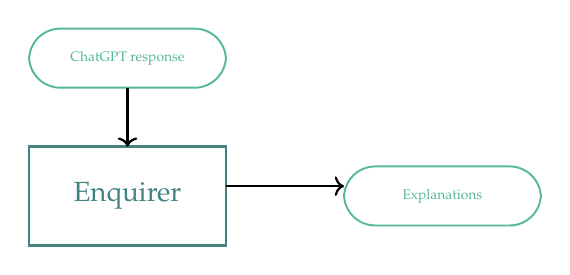
\begin{tikzpicture}
        \draw [ color={rgb,255:red,40; green,84; blue,154} , line width=1pt, visible on=<1->] (4,11.5) rectangle (6.5,10.25) node[pos=.5] {Enquirer};
        \draw [color={rgb,255:red,45; green,169; blue,155} , line width=0.7pt, rounded corners = 11.3, visible on=<3->] (8,10.5) rectangle (10.5,11.25) node[pos=.5] {\tiny{Explanations}};;
        % \draw [ color={rgb,255:red,40; green,84; blue,154} , line width=1pt ] (4.25,8) rectangle (6.25,6.5)  node[pos=.5] {\footnotesize{Challenger}};;;
        % \draw [ color={rgb,255:red,45; green,169; blue,155} , line width=0.7pt, rounded corners = 11.3] (8.25,7.5) rectangle (10.5,6.75) node[pos=.5] {\tiny{Challenge responses}};;;
        % \draw [ color={rgb,255:red,40; green,84; blue,154} , line width=1pt ] (12.5,10.25) rectangle (14.5,8.5) node[pos=.5] {Decider};;
        \draw [ color={rgb,255:red,45; green,169; blue,155} , line width=0.7pt, rounded corners = 11.3,visible on=<2->] (4,13) rectangle (6.5,12.25) node[pos=.5] {\tiny{ChatGPT response}};
        % \draw [ color={rgb,255:red,45; green,169; blue,155} , line width=0.7pt, rounded corners = 11.3] (11.75,12.5) rectangle (15,11.75) node[pos=.5] {\tiny{Explanation-wise correctness}};
        \draw [->, thick, visible on=<2->] (5.25,12.25) -- (5.25,11.5);
        \draw [->, thick, visible on=<3->] (6.5,11) -- (8,11);
        % \draw [short, thick] (9.25,10.5) -- (9.25,9.25);
        % \draw [short, thick] (9.25,9.25) -- (5.5,9.25);
        % \draw [->, thick] (5.5,9.25) -- (5.5,8);
        % \draw [->, thick] (6.25,7.25) -- (8.25,7.25);
        % \draw [->, thick] (10.5,7.25) -- (12.5,9.25);
        % \draw [->, thick] (10.5,10.75) -- (12.5,9.25);
        % \draw [->, thick] (13.5,10.25) -- (13.5,11.75);
    \end{tikzpicture}
\end{frame}

%------------------------------------------------

% \begin{frame}
%     \frametitle{CID Components}
%     \begin{figure}
%         \centering
%         \begin{tikzpicture}[node distance=1.5cm]
%             % Nodes
%             \node (start) [startstop] {Start};
%             \node (enquirer) [process, below of=start] {ENQUIRER};
%             \node (challenger) [process, below of=enquirer] {CHALLENGER};
%             \node (decider) [process, below of=challenger] {DECIDER};
%             \node (end) [startstop, below of=decider] {End};
%             % Arrows
%             \draw [arrow] (start) -- (enquirer);
%             \draw [arrow] (enquirer) -- (challenger);
%             \draw [arrow] (challenger) -- (decider);
%             \draw [arrow] (decider) -- (end);
%         \end{tikzpicture}
%         \caption{Overview of CID Tool Workflow}
%     \end{figure}
% \end{frame}

%------------------------------------------------

\begin{frame}
    \frametitle{ENQUIRER Component}
    \begin{itemize}
        \item \footnotesize{The ENQUIRER targets to obtain ChatGPT’s initial reasoning behind the
base-response that can be useful to reveal any inconsistency in
the next steps of interrogation.} \pause
        \item \footnotesize{Asks ChatGPT to provide separate reasoning for each piece of information by using the following prompt.} \pause
        \begin{center}
        \begin{minipage}{0.8\textwidth}
            \begin{block}{\footnotesize{Enquiring ChatGPT}}
                \footnotesize{Justify your answer. If the answer has multiple
pieces of information, provide separate reasoning for each of them.}
            \end{block}
        \end{minipage}
        \end{center}
    \end{itemize}
\end{frame}

% %------------------------------------------------

\begin{frame}{}
    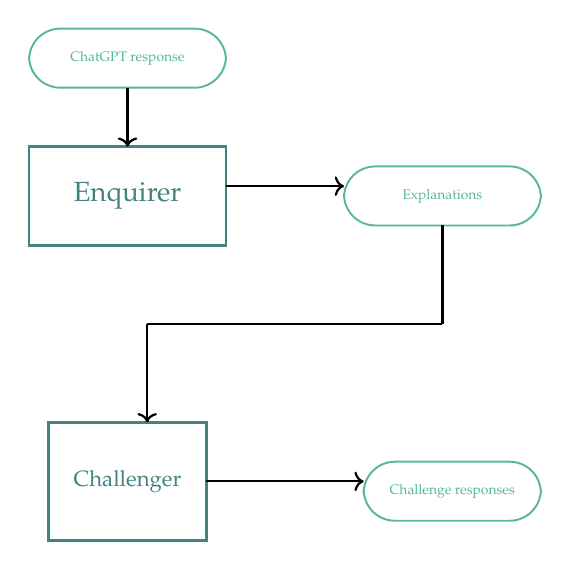
\begin{tikzpicture}
        \draw [ color={rgb,255:red,40; green,84; blue,154} , line width=1pt, visible on=<1->] (4,11.5) rectangle (6.5,10.25) node[pos=.5] {Enquirer};
        \draw [color={rgb,255:red,45; green,169; blue,155} , line width=0.7pt, rounded corners = 11.3, visible on=<1->] (8,10.5) rectangle (10.5,11.25) node[pos=.5] {\tiny{Explanations}};;
        \draw [ color={rgb,255:red,40; green,84; blue,154} , line width=1pt , visible on=<1->] (4.25,8) rectangle (6.25,6.5)  node[pos=.5] {\footnotesize{Challenger}};;;
        \draw [ color={rgb,255:red,45; green,169; blue,155} , line width=0.7pt, rounded corners = 11.3, visible on=<3->] (8.25,7.5) rectangle (10.5,6.75) node[pos=.5] {\tiny{Challenge responses}};;;
        % \draw [ color={rgb,255:red,40; green,84; blue,154} , line width=1pt ] (12.5,10.25) rectangle (14.5,8.5) node[pos=.5] {Decider};;
        \draw [ color={rgb,255:red,45; green,169; blue,155} , line width=0.7pt, rounded corners = 11.3,visible on=<1->] (4,13) rectangle (6.5,12.25) node[pos=.5] {\tiny{ChatGPT response}};
        % \draw [ color={rgb,255:red,45; green,169; blue,155} , line width=0.7pt, rounded corners = 11.3] (11.75,12.5) rectangle (15,11.75) node[pos=.5] {\tiny{Explanation-wise correctness}};
        \draw [->, thick, visible on=<1->] (5.25,12.25) -- (5.25,11.5);
        \draw [->, thick, visible on=<1->] (6.5,11) -- (8,11);
        \draw [short, thick, visible on=<2->] (9.25,10.5) -- (9.25,9.25);
        \draw [short, thick, visible on=<2->] (9.25,9.25) -- (5.5,9.25);
        \draw [->, thick, visible on=<2->] (5.5,9.25) -- (5.5,8);
        \draw [->, thick, visible on=<3->] (6.25,7.25) -- (8.25,7.25);
        % \draw [->, thick] (10.5,7.25) -- (12.5,9.25);
        % \draw [->, thick] (10.5,10.75) -- (12.5,9.25);
        % \draw [->, thick] (13.5,10.25) -- (13.5,11.75);
    \end{tikzpicture}
\end{frame}

\begin{frame}{Challenger Components}
    \begin{center} % Center the entire tikzpicture
        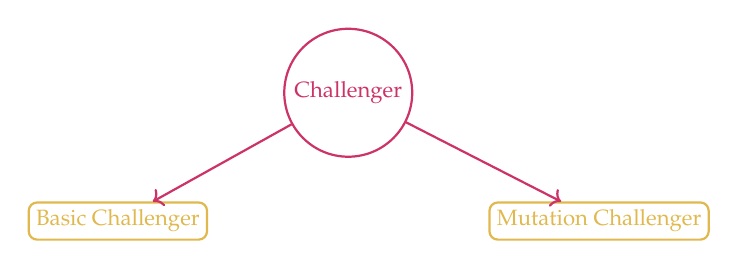
\begin{tikzpicture}[scale=0.8, every node/.style={transform shape}]
            % Main Challenger node
            \node[draw, circle, minimum size=0.8cm, thick, color=purple!80, visible on=<1->] (Challenger) at (0, 2) {Challenger};

            % Basic Challenger node (red)
            \node[draw, rectangle, rounded corners=3pt, thick, color=goldenrod!80, below left=1cm and 1.5cm of Challenger, visible on=<2->] (Basic) {Basic Challenger};

            % Mutation Challenger node (purple)
            \node[draw, rectangle, rounded corners=3pt, thick, color=goldenrod!80, below right=1cm and 1.5cm of Challenger, visible on=<3->] (Mutation) {Mutation Challenger};

            % Connecting arrows
            \draw[->, thick, color=purple!80, visible on=<2->] (Challenger) -- (Basic);
            \draw[->, thick, color=purple!80, visible on=<3->] (Challenger) -- (Mutation);
        \end{tikzpicture}
    \end{center}
\end{frame}

\begin{frame}
    \frametitle{Basic Challenger}
    \begin{itemize}
        \item \footnotesize{We first ask three basic challenge questions
to ChatGPT: \emph{Why?, How?, Really?} for each explanation $(E_i
)$ of its
base-response $(R_B)$.}
        \pause
        \item \footnotesize{The basic challenger leverages a separate LLM. } \pause
        \item \footnotesize{To replicate a separate LLM, we used ChatGPT with a new separate
session. The motive for using a separate session of ChatGPT is
to discard the memory of the previous conversation performed.}
    \end{itemize}
\end{frame}

\begin{frame}
    \frametitle{Mutation Challenger}
    \begin{itemize}
        \item \footnotesize{Aims to increase the cognitive load of the model.}
        \pause
        \item \footnotesize{It mutates the basic challenge questions to
create mutation challenge questions. } \pause
        \item \footnotesize{Employs the \emph{Sentence-level metamorphic testing technique,
QAQA}}
        \pause
        \item \footnotesize{It inserts a redundant sentence as a clause
to the original (basic challenge) question to generate the mutated
question and challenges it.}
        \pause
        \item \footnotesize{Depending on the source of the redundant sentence,
the mutation challenger applies two types of metamorphic relation
(MR): \textbf{Equivalent Question (MR1)} and \textbf{Equivalent Test Integration (MR2)}}
    \end{itemize}
\end{frame}

\begin{frame}{Mutated Questions Flow Example}
    \begin{center}
        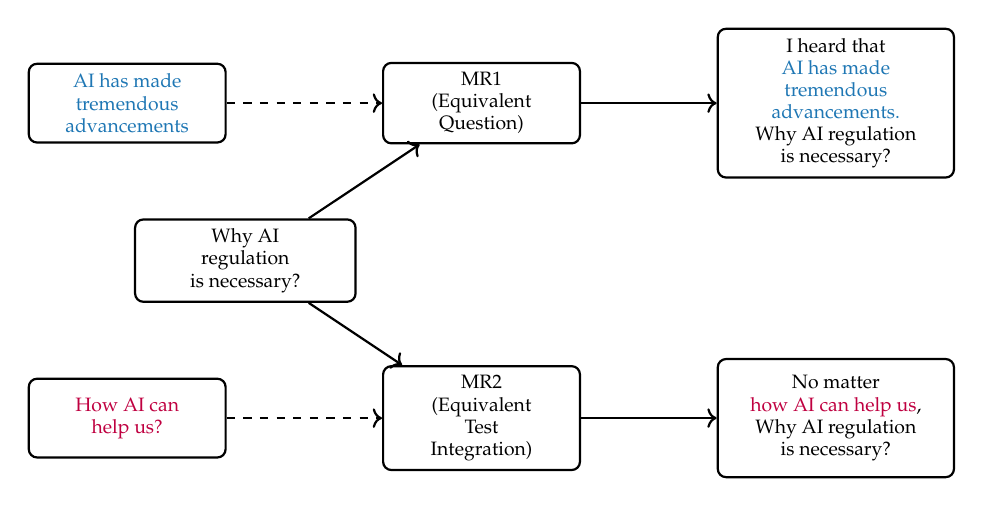
\begin{tikzpicture}[
            every node/.style={align=center},
            rect/.style={draw, rectangle, rounded corners=3pt, thick, font=\scriptsize},
            arrow/.style={->, thick},
            dashed_arrow/.style={->, thick, dashed}
        ]

            % Nodes
            \node[rect, minimum width=2.5cm, minimum height=1cm, visible on=<3->] (info1) at (-3, 2.5) {\textcolor{blue}{AI has made} \\ \textcolor{blue}{tremendous} \\ \textcolor{blue}{advancements}};
            \node[rect, minimum width=2.5cm, minimum height=1cm, visible on=<5->] (info2) at (-3, -1.5) {\textcolor{purple}{How AI can} \\ \textcolor{purple}{help us?}};

            \node[rect, minimum width=2.8cm, minimum height=1cm, visible on=<1->] (basic) at (-1.5, 0.5) {Why AI \\ regulation \\ is necessary?};
            
            \node[rect, minimum width=2.5cm, minimum height=1cm, visible on=<2->] (mr1) at (1.5, 2.5) {MR1 \\ (Equivalent \\ Question)};
            \node[rect, minimum width=2.5cm, minimum height=1cm, visible on=<2->] (mr2) at (1.5, -1.5) {MR2 \\ (Equivalent \\ Test \\ Integration)};
            
            \node[rect, minimum width=3cm, minimum height=1.5cm, visible on=<4->] (mut1) at (6, 2.5) {
                I heard that \\ \textcolor{blue}{AI has made} \\ \textcolor{blue}{tremendous}
                \\ \textcolor{blue}{advancements.} \\ Why AI regulation \\ is necessary?
            };
            \node[rect, minimum width=3cm, minimum height=1.5cm, visible on=<6->] (mut2) at (6, -1.5) {
                No matter \\ \textcolor{purple}{how AI can help us}, \\ Why AI regulation \\ is necessary?
            };

            % Connections
            \draw[dashed_arrow, visible on=<3->] (info1) -- (mr1);
            \draw[dashed_arrow, visible on=<5->] (info2) -- (mr2);
            \draw[arrow, visible on=<2->] (basic) -- (mr1);
            \draw[arrow, visible on=<2->] (basic) -- (mr2);
            \draw[arrow, visible on=<4->] (mr1) -- (mut1);
            \draw[arrow, visible on=<6->] (mr2) -- (mut2);

        \end{tikzpicture}
    \end{center}
\end{frame}



\begin{frame}{}
    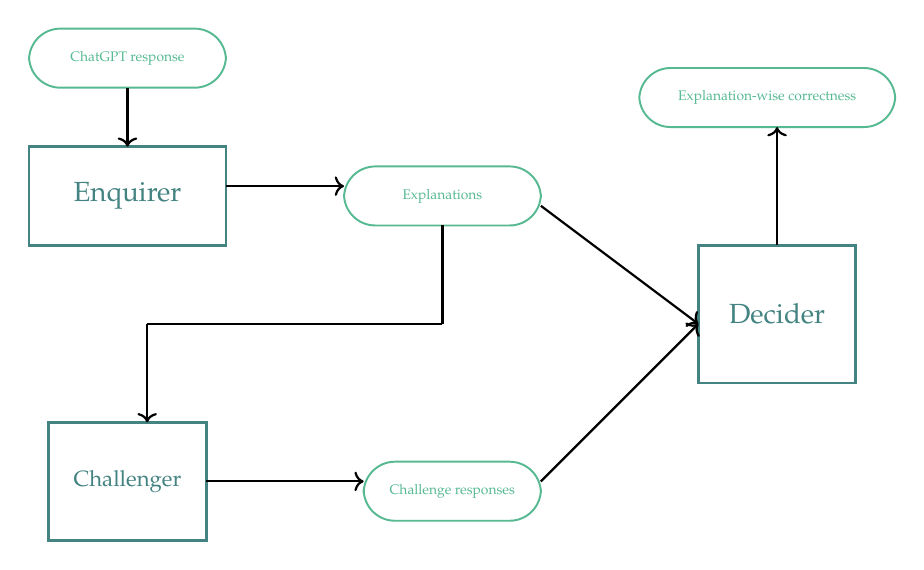
\begin{tikzpicture}
        \draw [ color={rgb,255:red,40; green,84; blue,154} , line width=1pt, visible on=<1->] (4,11.5) rectangle (6.5,10.25) node[pos=.5] {Enquirer};
        \draw [color={rgb,255:red,45; green,169; blue,155} , line width=0.7pt, rounded corners = 11.3, visible on=<1->] (8,10.5) rectangle (10.5,11.25) node[pos=.5] {\tiny{Explanations}};;
        \draw [ color={rgb,255:red,40; green,84; blue,154} , line width=1pt , visible on=<1->] (4.25,8) rectangle (6.25,6.5)  node[pos=.5] {\footnotesize{Challenger}};;;
        \draw [ color={rgb,255:red,45; green,169; blue,155} , line width=0.7pt, rounded corners = 11.3, visible on=<1->] (8.25,7.5) rectangle (10.5,6.75) node[pos=.5] {\tiny{Challenge responses}};;;
        \draw [ color={rgb,255:red,40; green,84; blue,154} , line width=1pt, visible on=<2-> ] (12.5,10.25) rectangle (14.5,8.5) node[pos=.5] {Decider};;
        \draw [ color={rgb,255:red,45; green,169; blue,155} , line width=0.7pt, rounded corners = 11.3,visible on=<1->] (4,13) rectangle (6.5,12.25) node[pos=.5] {\tiny{ChatGPT response}};
        \draw [ color={rgb,255:red,45; green,169; blue,155} , line width=0.7pt, rounded corners = 11.3, visible on=<3->] (11.75,12.5) rectangle (15,11.75) node[pos=.5] {\tiny{Explanation-wise correctness}};
        \draw [->, thick, visible on=<1->] (5.25,12.25) -- (5.25,11.5);
        \draw [->, thick, visible on=<1->] (6.5,11) -- (8,11);
        \draw [short, thick, visible on=<1->] (9.25,10.5) -- (9.25,9.25);
        \draw [short, thick, visible on=<1->] (9.25,9.25) -- (5.5,9.25);
        \draw [->, thick, visible on=<1->] (5.5,9.25) -- (5.5,8);
        \draw [->, thick, visible on=<1->] (6.25,7.25) -- (8.25,7.25);
        \draw [->, thick, visible on=<2->] (10.5,7.25) -- (12.5,9.25);
        \draw [->, thick, visible on=<2->] (10.5,10.75) -- (12.5,9.25);
        \draw [->, thick, , visible on=<3->] (13.5,10.25) -- (13.5,11.75);
    \end{tikzpicture}
\end{frame}

\begin{frame}{Decider Modules}
    \begin{center} % Center the entire tikzpicture
        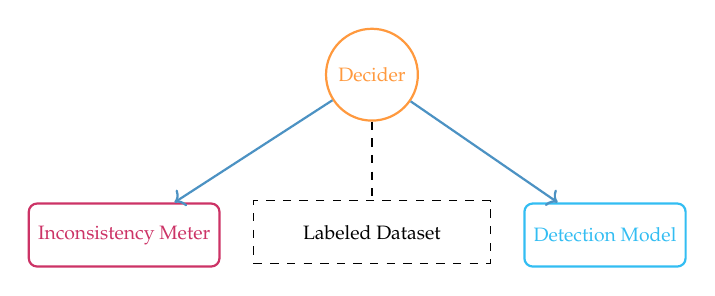
\begin{tikzpicture}
            % Main Decider node
            \node[draw, circle, minimum size=0.6cm, thick, color=orange!80, font=\scriptsize, visible on=<1->] (Decider) at (0, 2) {Decider};

            % Inconsistency Meter node (green)
            \node[draw, rectangle, rounded corners=3pt, thick, color=purple!80, minimum width=2cm, minimum height=0.8cm, font=\scriptsize, below left=1.2cm and 1.5cm of Decider, , visible on=<2->] (Inconsistency) {Inconsistency Meter};

            % Dataset Creation node (orange)
            \node[draw, rectangle, rounded corners=3pt, thick, color=cyan!80, minimum width=2cm, minimum height=0.8cm, font=\scriptsize, below right=1.2cm and 1.5cm of Decider, visible on=<3->] (Dataset) {Detection Model};

            % Labeled Dataset (Dashed box)
            \node[draw, dashed, minimum width=3cm, minimum height=0.8cm, font=\scriptsize, visible on=<4->] (Labeled) at (0, 0) {Labeled Dataset};

            % Connecting arrows (pointing downward)
            \draw[->, thick, color=blue!80, , visible on=<2->] (Decider) -- (Inconsistency);
            \draw[->, thick, color=blue!80, , visible on=<3->] (Decider) -- (Dataset);
            \draw[dashed, thick, , visible on=<4->] (Decider) -- (Labeled);
        \end{tikzpicture}
    \end{center}
\end{frame}
% \begin{frame}
%     \frametitle{DECIDER Component}
%     \begin{itemize}
%         \item Analyzes responses for inconsistencies.
%         \item Employs similarity measures and machine learning models.
%         \item Determines correctness based on detected inconsistencies.
%         \item Features Used:
%         \begin{itemize}
%             \item Explanation-Response Similarity
%             \item Response-Response Similarity
%             \item Question-Response Similarity
%             \item Question-Question Similarity
%         \end{itemize}
%     \end{itemize}
% \end{frame}

\begin{frame}
    \frametitle{Dataset Creation}
    \begin{itemize}
        \item \footnotesize{The dataset is generated by interacting with ChatGPT and posing various questions to it.}
        \pause
        \item \footnotesize{we use our ENQUIRER to split each base response into multiple
explanations. Finally, these explanations are manually labeled
as correct/incorrect by human annotators.} 
    \end{itemize}
\end{frame}

\begin{frame}
    \frametitle{Inconsistency Meter and Detection Model}
    \begin{itemize}
        \item \footnotesize{Standard similarity scores is computed among ChatGPT responses generated
in the ENQUIRY and CHALLENGE phases.}
        \pause
        \item \footnotesize{These scores are used as features
for our tool.} 
        \pause 
        \item \footnotesize{ML model is trained so that they learn the relationship between ChatGPT's incorrectness and inconsistency.} 
        \pause 
        \item \footnotesize{$24$ features from four categories is used to train the model.} 
        \begin{itemize}
            \item \footnotesize{Explanation-Response $(E_{i}-R_{C})$ Similarity}
            \item \footnotesize{Response-Response $(R_{C}-R_{C})$ Similarity}
            \item \footnotesize{Question-Response $(Q_{C}-R_{C})$ Similarity}
            \item \footnotesize{Question-Question $(Q_{C}-Q_{C})$ Similarity}
        \end{itemize}
    \end{itemize}
\end{frame}

\begin{frame}{CID Tool Overview}
    \begin{center}
        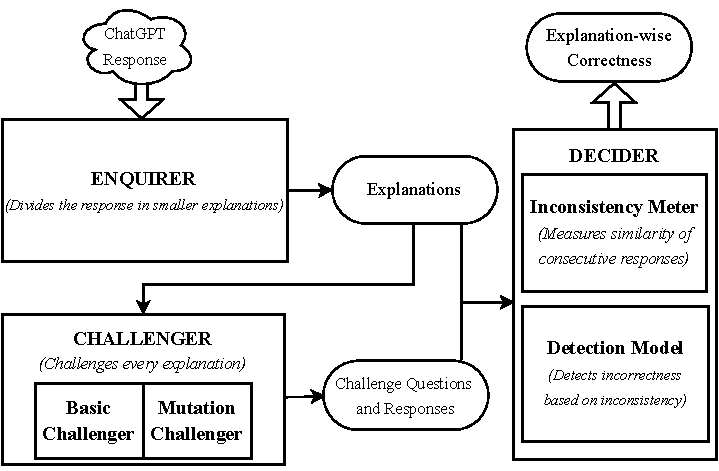
\includegraphics[width=0.8\textwidth]{modules/nafees/CID_tool_overview.pdf}
    \end{center}
\end{frame}
%------------------------------------------------
%----------------------------------
% Evaluation of CID Section
%----------------------------------
\section{Evaluation of CID}

% Slide: Evaluation of CID Introduction
\begin{frame}
  \frametitle{Evaluation of CID}
  \begin{itemize}
    \item \textbf{Research Questions}
    \begin{itemize}
      \item \textbf{RQ4}: How accurate is CID in detecting incorrect responses?
      \item \textbf{RQ5}: How do the base and mutation challenge prompts impact performance?
    \end{itemize}
  \end{itemize}
\end{frame}

% Slide: Benchmark Study Setup
\begin{frame}
  \frametitle{Benchmark Study Setup}
  \begin{itemize}
    \item \textbf{Context}: Software Library Selection Task
    \item \textbf{Dataset Collection}:
    \begin{itemize}
      \item Collected 100 Stack Overflow (SO) posts
      \item Focused on text processing libraries: \textbf{spaCy}, \textbf{NLTK}, \textbf{GSON}
      \item Covered aspects like ease of use, performance, stability, etc.
    \end{itemize}
    \item \textbf{Base Questions}:
    \begin{itemize}
      \item Formulated questions based on SO posts
      \item Example: \textit{"How easy is it to use the library strictly based on the following conversation?"}
    \end{itemize}
  \end{itemize}
\end{frame}

% Slide: Visualizing the Benchmark Setup
\begin{frame}
  \frametitle{Visualizing the Benchmark Setup}
  \begin{center}
    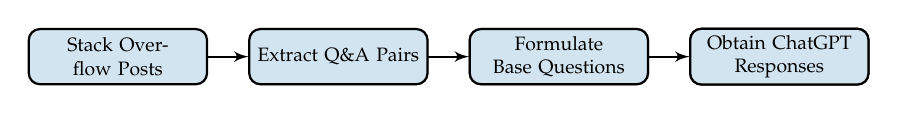
\begin{tikzpicture}[node distance=2cm, auto, thick, scale=0.7, transform shape]
      % Define styles for active and inactive nodes
      \tikzstyle{activeblock} = [rectangle, draw, fill=blue!20, text width=3cm, text centered, rounded corners, minimum height=1cm, opacity=1]
      \tikzstyle{inactiveblock} = [rectangle, draw, fill=blue!20, text width=3cm, text centered, rounded corners, minimum height=1cm, opacity=0.3]
      \tikzstyle{activeline} = [draw, -latex', opacity=1]
      \tikzstyle{inactiveline} = [draw, -latex', opacity=0.3]
      
      % Nodes
      \node<1-4> [activeblock] (posts) {Stack Overflow Posts};
      \node<1> [inactiveblock, right of=posts, node distance=4cm] (extract) {Extract Q\&A Pairs};
      \node<1> [inactiveblock, right of=extract, node distance=4cm] (questions) {Formulate Base Questions};
      \node<1> [inactiveblock, right of=questions, node distance=4cm] (chatgpt) {Obtain ChatGPT Responses};

      \node<2-4> [activeblock, right of=posts, node distance=4cm] (extract) {Extract Q\&A Pairs};
      \node<2> [inactiveblock, right of=extract, node distance=4cm] (questions) {Formulate Base Questions};
      \node<2> [inactiveblock, right of=questions, node distance=4cm] (chatgpt) {Obtain ChatGPT Responses};

      \node<3-4> [activeblock, right of=extract, node distance=4cm] (questions) {Formulate Base Questions};
      \node<3> [inactiveblock, right of=questions, node distance=4cm] (chatgpt) {Obtain ChatGPT Responses};

      \node<4> [activeblock, right of=questions, node distance=4cm] (chatgpt) {Obtain ChatGPT Responses};

      % Arrows
      \path<1> [inactiveline] (posts) -- (extract);
      \path<2-4> [activeline] (posts) -- (extract);
      
      \path<1-2> [inactiveline] (extract) -- (questions);
      \path<3-4> [activeline] (extract) -- (questions);
      
      \path<1-3> [inactiveline] (questions) -- (chatgpt);
      \path<4> [activeline] (questions) -- (chatgpt);
    \end{tikzpicture}
    \captionof{figure}{Flowchart of Benchmark Study Setup}
  \end{center}
\end{frame}



% Slide: CID Components Diagram
\begin{frame}
  \frametitle{CID Components Recap}

    % Items at the top for each overlay
      \only<1>{
      \textbf{ENQUIRER}
      \begin{itemize}
        \item Extracts explanations from ChatGPT's base responses
      \end{itemize}
      }
      \only<2>{
      \textbf{CHALLENGER} 
      \begin{itemize}
        \item Poses basic and mutated challenge questions
        \item Uses metamorphic relationships to mutate questions
      \end{itemize}
      }
      \only<3>{\textbf{DECIDER}
      \begin{itemize}
        \item Analyzes inconsistencies
        \item Employs ML techniques to detect incorrectness
      \end{itemize}
      }
  
    \vspace{0.5cm} % Add some space between items and diagram

  \begin{center}
    \begin{tikzpicture}[node distance=3cm, auto, thick, scale=0.6, transform shape]
      % Define styles for active and inactive nodes
      \tikzstyle{activeblock} = [rectangle, draw, fill=blue!20, text width=2.8cm, text centered, rounded corners, minimum height=1cm, opacity=1]
      \tikzstyle{inactiveblock} = [rectangle, draw, fill=blue!20, text width=2.8cm, text centered, rounded corners, minimum height=1cm, opacity=0.3]
      \tikzstyle{activeline} = [draw, -latex', opacity=1]
      \tikzstyle{inactiveline} = [draw, -latex', opacity=0.3]

      % Nodes and Arrows with Overlays
      % Overlay 1: Highlight Enquirer
      \only<1>{
        \node [activeblock] (enquirer) {Enquirer};
        \node [inactiveblock, right=of enquirer, xshift=1cm] (challenger) {Challenger};
        \node [inactiveblock, right=of challenger, xshift=1cm] (decider) {Decider};

        \path [inactiveline] (enquirer) -- node [above, yshift=0.2cm] {Explanations} (challenger);
        \path [inactiveline] (challenger) -- node [above, yshift=0.2cm] {Challenge Responses} (decider);
        \draw [inactiveline] (decider.south) |- ++(0,-1.5cm) -| node [below, pos=0.5, yshift=-0.2cm, xshift=7.1cm] {Feedback} (enquirer.south);
      }

      % Overlay 2: Highlight Enquirer and Challenger
      \only<2>{
        \node [activeblock] (enquirer) {Enquirer};
        \node [activeblock, right=of enquirer, xshift=1cm] (challenger) {Challenger};
        \node [inactiveblock, right=of challenger, xshift=1cm] (decider) {Decider};

        \path [activeline] (enquirer) -- node [above, yshift=0.2cm] {Explanations} (challenger);
        \path [inactiveline] (challenger) -- node [above, yshift=0.2cm] {Challenge Responses} (decider);
        \draw [inactiveline] (decider.south) |- ++(0,-1.5cm) -| node [below, pos=0.5, yshift=-0.2cm, xshift=7.1cm] {Feedback} (enquirer.south);
      }

      % Overlay 3: Highlight all components
      \only<3>{
        \node [activeblock] (enquirer) {Enquirer};
        \node [activeblock, right=of enquirer, xshift=1cm] (challenger) {Challenger};
        \node [activeblock, right=of challenger, xshift=1cm] (decider) {Decider};

        \path [activeline] (enquirer) -- node [above, yshift=0.2cm] {Explanations} (challenger);
        \path [activeline] (challenger) -- node [above, yshift=0.2cm] {Challenge Responses} (decider);
        \draw [activeline] (decider.south) |- ++(0,-1.5cm) -| node [below, pos=0.5, yshift=-0.2cm, xshift=7.1cm] {Feedback} (enquirer.south);
      }

    \end{tikzpicture}
    \captionof{figure}{Interaction between CID Components}
  \end{center}
\end{frame}




% Slide: Explanation Generation (Text)
\begin{frame}
  \frametitle{Explanation Generation}
    \textbf{Process}:
    \begin{itemize}
      \item ChatGPT provides base responses to base questions
      \item ENQUIRER requests separate explanations for each piece of information
    \end{itemize}
\end{frame}

% Slide: Explanation Generation (Figure)
\begin{frame}
  \frametitle{Explanation Generation}
  \vspace{0.5cm}
  \textbf{Outcome}:
    \begin{itemize}
      \item Generated 341 explanations from 100 posts
      \item \textbf{Labeling}:
      \begin{itemize}
        \item \only<1>{\textbf{\textcolor{mygreen}{276 explanations (81\%) labeled as correct}}}
              \only<2>{\textcolor{mygreen!20}{276 explanations (81\%) labeled as correct}}
        \item \only<2>{\textbf{\textcolor{myred}{65 explanations (19\%) labeled as incorrect}}}
              \only<1>{\textcolor{myred!20}{65 explanations (19\%) labeled as incorrect}}
      \end{itemize}
    \end{itemize}
  \begin{center}
    \begin{tikzpicture}[scale=0.5, transform shape]
      % First overlay: Highlight Correct Explanations
      \only<1>{
        \pie[
          color = {mygreen!70, myred!15},
          explode = {0.1, 0},
          text = legend,
          sum = 100,
        ]{81/Correct Explanations, 19/Incorrect Explanations}
      }
      % Second overlay: Highlight Incorrect Explanations
      \only<2>{
        \pie[
          color = {mygreen!15, myred!70},
          explode = {0, 0.1},
          text = legend,
          sum = 100,
        ]{81/Correct Explanations, 19/Incorrect Explanations}
      }
    \end{tikzpicture}
    \captionof{figure}{Distribution of Correct and Incorrect Explanations}
  \end{center}
\end{frame}






% Slide: Incorrectness Detection Performance (RQ4) (Text)
\begin{frame}
  \frametitle{Incorrectness Detection Performance (RQ4)}
  \begin{itemize}
    \item \textbf{Machine Learning Models Evaluated}:
    \begin{itemize}
      \item Logistic Regression (LR)
      \item Random Forest (RF)
      \item Support Vector Machine (SVM)
    \end{itemize}
    \item \textbf{Performance Metrics}:
    \begin{itemize}
      \item Precision (P), Recall (R), F1-Score (F1), Accuracy (A)
    \end{itemize}
  \end{itemize}
  % \vspace{0.2cm}
  \begin{center}
    \small
    \begin{tabular}{lrrrr}
    \toprule
     \textbf{Model} & \textbf{P} & \textbf{R} & \textbf{A} & \textbf{F1} \\ \midrule
    Logistic Regression (LR) & 0.74 & 0.65 & 0.65 & 0.68 \\ 
    Random Forest (RF) & 0.73 & 0.65 & 0.65 & 0.68 \\ 
    Support Vector Machine (SVM) & \textbf{0.74} & \textbf{0.75} & \textbf{0.75} & \textbf{0.74} \\ 
    \bottomrule
    \end{tabular}
    \captionof{table}{ML model performance to detect ChatGPT incorrectness}
    \label{tab:model_accuracy}
  \end{center}
\end{frame}


% Slide: Visualizing Model Performance
\begin{frame}
  \frametitle{Visualizing Model Performance}
  \begin{center}
    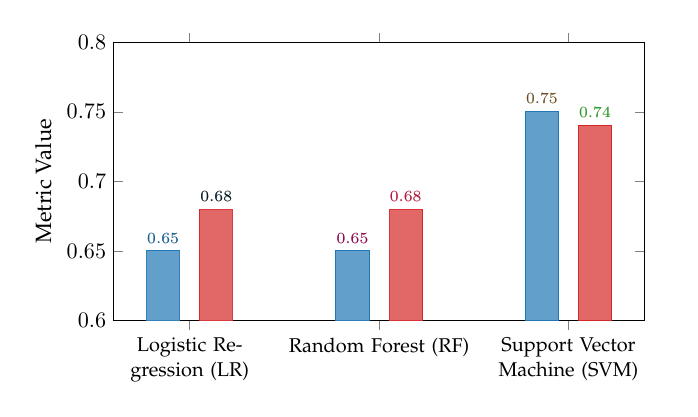
\begin{tikzpicture}[scale=0.8,transform shape]
    \begin{axis}[
      ybar,
      bar width=15pt, % Increased bar width
      width=10cm,
      height=6cm,
      enlarge x limits=0.2,
      legend style={
        at={(0.5,-0.25)},
        anchor=north,
        legend columns=2
      },
      symbolic x coords={LR, RF, SVM},
      xtick={LR, RF, SVM}, % Explicitly set x-axis ticks
      xticklabels={Logistic Regression (LR), Random Forest (RF), Support Vector Machine (SVM)},
      x tick label style={
        text width=3cm,
        align=center,
        font=\small,
      },
      ylabel={Metric Value},
      ymin=0.6, ymax=0.8,
      nodes near coords,
      nodes near coords align={vertical},
      every node near coord/.append style={font=\scriptsize}, % Smaller font size
    ]


  
        % Data for Accuracy (Blue Bars)
        \addplot+[
          draw=blue, fill=blue!70,
          bar shift=-12pt, % Increased spacing between red and blue bars
          opacity=1, % Fully opaque for highlighted bar
          visible on=<1>
        ] coordinates {(LR,0.65)};
        \addplot+[
          draw=blue, fill=blue!70,
          bar shift=-12pt,
          opacity=0.3, % Less opaque for non-highlighted bars
          visible on=<1>
        ] coordinates {(RF,0.65)};
        \addplot+[
          draw=blue, fill=blue!70,
          bar shift=-12pt,
          opacity=0.3,
          visible on=<1>
        ] coordinates {(SVM,0.75)};
  
        % Highlight RF on Slide 2
        \addplot+[
          draw=blue, fill=blue!70,
          bar shift=-12pt,
          opacity=0.3,
          visible on=<2>
        ] coordinates {(LR,0.65)};
        \addplot+[
          draw=blue, fill=blue!70,
          bar shift=-12pt,
          opacity=1,
          visible on=<2>
        ] coordinates {(RF,0.65)};
        \addplot+[
          draw=blue, fill=blue!70,
          bar shift=-12pt,
          opacity=0.3,
          visible on=<2>
        ] coordinates {(SVM,0.75)};
  
        % Highlight SVM on Slide 3
        \addplot+[
          draw=blue, fill=blue!70,
          bar shift=-12pt,
          opacity=0.3,
          visible on=<3>
        ] coordinates {(LR,0.65)};
        \addplot+[
          draw=blue, fill=blue!70,
          bar shift=-12pt,
          opacity=0.3,
          visible on=<3>
        ] coordinates {(RF,0.65)};
        \addplot+[
          draw=blue, fill=blue!70,
          bar shift=-12pt,
          opacity=1,
          visible on=<3>
        ] coordinates {(SVM,0.75)};
  
        % Data for F1-Score (Red Bars)
        \addplot+[
          draw=red, fill=red!70,
          bar shift=12pt, % Increased spacing between red and blue bars
          opacity=1,
          visible on=<1>
        ] coordinates {(LR,0.68)};
        \addplot+[
          draw=red, fill=red!70,
          bar shift=12pt,
          opacity=0.3,
          visible on=<1>
        ] coordinates {(RF,0.68)};
        \addplot+[
          draw=red, fill=red!70,
          bar shift=12pt,
          opacity=0.3,
          visible on=<1>
        ] coordinates {(SVM,0.74)};
  
        % Highlight RF on Slide 2
        \addplot+[
          draw=red, fill=red!70,
          bar shift=12pt,
          opacity=0.3,
          visible on=<2>
        ] coordinates {(LR,0.68)};
        \addplot+[
          draw=red, fill=red!70,
          bar shift=12pt,
          opacity=1,
          visible on=<2>
        ] coordinates {(RF,0.68)};
        \addplot+[
          draw=red, fill=red!70,
          bar shift=12pt,
          opacity=0.3,
          visible on=<2>
        ] coordinates {(SVM,0.74)};
  
        % Highlight SVM on Slide 3
        \addplot+[
          draw=red, fill=red!70,
          bar shift=12pt,
          opacity=0.3,
          visible on=<3>
        ] coordinates {(LR,0.68)};
        \addplot+[
          draw=red, fill=red!70,
          bar shift=12pt,
          opacity=0.3,
          visible on=<3>
        ] coordinates {(RF,0.68)};
        \addplot+[
          draw=red, fill=red!70,
          bar shift=12pt,
          opacity=1,
          visible on=<3>
        ] coordinates {(SVM,0.74)};
  
        % Legends for Metrics (Appears on Slide 3)
        \only<3>{
          \addlegendimage{draw=blue,fill=blue!70}
          \addlegendentry{Accuracy}
          \addlegendimage{draw=red,fill=red!70}
          \addlegendentry{F1-Score}
          \legend{}
        }
  
      \end{axis}
    \end{tikzpicture}
    \captionof{figure}{Comparison of ML Model Performances}
  \end{center}
\end{frame}

% Slide: Misclassification Analysis (Donut Chart)
\begin{frame}
  \frametitle{Misclassification Analysis}

  \begin{itemize}
    \item \textbf{Total Misclassifications}: 86 out of 341 explanations
  \end{itemize}

  \only<2-5>{\begin{itemize}
    \item \textbf{Error Sources} (44\% of errors)
    \begin{itemize}
      \only<2>{\item 
        \textbf{Decider Component} (44\% of errors)
        \begin{itemize}
          \item Similarity calculation issues
          \item Difficulty detecting unanimous incorrect responses
        \end{itemize}
      }
      \only<3>{\item 
        \textbf{Challenger Component} (32\% of errors)
        \begin{itemize}
          \item Misdirected challenges
          \item Out-of-scope questions
        \end{itemize}
      }
      \only<4>{\item 
        \textbf{Enquirer Component} (5\% of errors)
        \begin{itemize}
          \item Convoluted explanations with multiple opinions
        \end{itemize}
      }
      \only<5>{\item 
        \textbf{Mixed Sources} (19\% of errors)
        \begin{itemize}
          \item Continuous incorrect reasoning by ChatGPT
          \item Generic issues (unclear information)
        \end{itemize}
      }
    \end{itemize}
  \end{itemize}}
  

  \centering % Center the content
  \vspace{0.5cm}
  \begin{center}
  % Define colors within the frame
  \begin{tikzpicture}[scale=0.5, transform shape]
    % Local color definitions
    \definecolor{DeciderColor}{RGB}{102, 102, 238}    % Blue
    \definecolor{ChallengerColor}{RGB}{119, 209, 243}  % Green
    \definecolor{EnqColor}{RGB}{241, 230, 145}        % Orange
    \definecolor{MixedColor}{RGB}{244, 182, 114}     % Purple
    \definecolor{GreyColor}{RGB}{192, 192, 192}     % Grey for blurred slices

    % Overlay 1: Highlight Decider
    \only<1>{
        \pie[
      cloud,
      text=inside,
      scale font,
      radius=3, % Increased radius for more space
      % Optionally adjust font size
      color={
          DeciderColor,
          ChallengerColor,
          EnqColor,
          MixedColor
        },
      font=\scriptsize
    ]{
      44/Decider,
      32/Challenger,
      5/Enq., % Abbreviated label
      19/Mixed
    }
    }
    \only<2>{
      \pie[
        cloud,
        text=inside,
        scale font,
        radius=3,
        color={
          DeciderColor,
          GreyColor,
          GreyColor,
          GreyColor
        },
        font=\scriptsize
      ]{
        44/Decider,
        32/Challenger,
        5/Enq.,
        19/Mixed
      }
    }

    % Overlay 2: Highlight Challenger
    \only<3>{
      \pie[
        cloud,
        text=inside,
        scale font,
        radius=3,
        color={
          GreyColor,
          ChallengerColor,
          GreyColor,
          GreyColor
        },
        font=\scriptsize
      ]{
        44/Decider,
        32/Challenger,
        5/Enq.,
        19/Mixed
      }
    }

    % Overlay 3: Highlight Enquirer
    \only<4>{
      \pie[
        cloud,
        text=inside,
        scale font,
        radius=3,
        color={
          GreyColor,
          GreyColor,
          EnqColor,
          GreyColor
        },
        font=\scriptsize
      ]{
        44/Decider,
        32/Challenger,
        5/Enq.,
        19/Mixed
      }
    }

    % Overlay 4: Highlight Mixed
    \only<5>{
      \pie[
        cloud,
        text=inside,
        scale font,
        radius=3,
        color={
          GreyColor,
          GreyColor,
          GreyColor,
          MixedColor
        },
        font=\scriptsize
      ]{
        44/Decider,
        32/Challenger,
        5/Enq.,
        19/Mixed
      }
    }
  \end{tikzpicture}
\end{center}

  % Caption below the chart
  \captionof{figure}{Distribution of Error Sources}

\end{frame}


% Slide: Impact of Challenge Prompts (RQ5) (Text)
% Slide: Impact of Challenge Prompts (Merged)
\begin{frame}
  \frametitle{Impact of Challenge Prompts (RQ5)}

  % Slide 1: Experiment Setup

    \begin{itemize}
      \item \textbf{Experiment Setup}:
      \begin{itemize}
        \item Evaluated the impact of individual challenge prompts
        \item Tested performance by excluding each question type
      \end{itemize}
    \end{itemize}


  % Slide 2: Table of Results
    \begin{center}
      \small
      \begin{tabular}{lrr}
      \toprule
      \textbf{Scenarios} & \textbf{Accuracy} & \textbf{F1-score} \\ \midrule
      With all questions & 0.75 & 0.74 \\
      Without \textit{How} questions & 0.75 & 0.75 \\
      Without \textit{Really} questions & 0.69 & 0.70 \\ 
      Without \textit{Why} questions & 0.70 & 0.71 \\ 
      \bottomrule         
      \end{tabular}
      \captionof{table}{Impact of individual challenge prompts}
      \label{tab:challenge_question_impact}
    \end{center}
\end{frame}


% Slide: Visualizing Impact of Challenge Prompts
\begin{frame}
  \frametitle{Visualizing Impact of Challenge Prompts}
  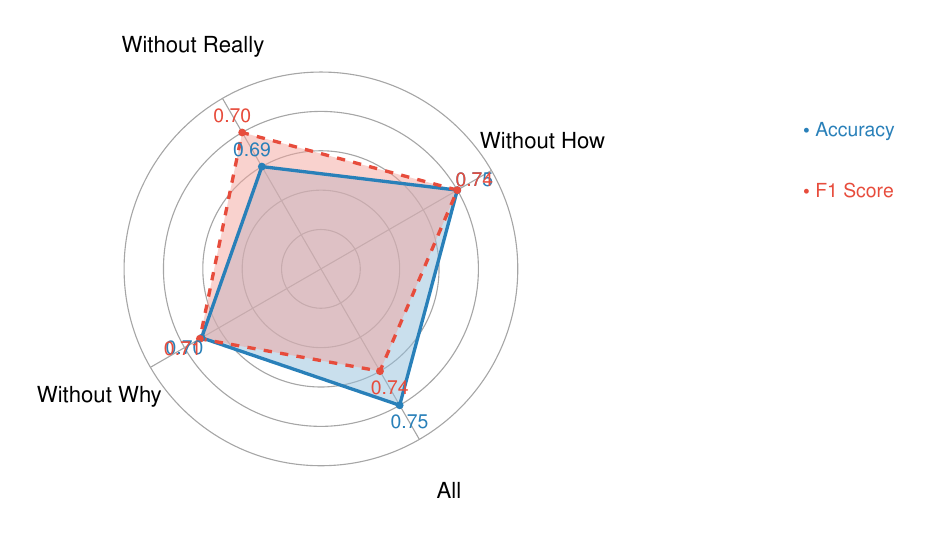
\begin{tikzpicture}[scale=0.5]
      % Color definitions
      \definecolor{accuracycolor}{RGB}{41, 128, 185}
      \definecolor{f1color}{RGB}{231, 76, 60}
      
      % Radar chart parameters
      \def\maxradius{5}
      
      % Draw background grid
      \foreach \r in {1,2,3,4,5} {
          \draw[gray!70] (0,0) circle (\r);
      }
      
      % Draw axes
      \foreach \angle/\label in {
          30/Without How, 
          120/Without Really, 
          210/Without Why, 
          300/All
      } {
          \draw[gray!70] (\angle:\maxradius) -- (\angle:0);
          \node[font=\footnotesize\sffamily] at (\angle:\maxradius+1.5) {\label};
      }
      
      % Accuracy values (scaled by 5)
      \def\accuracyWithoutHow{4}
      \def\accuracyWithoutReally{3}
      \def\accuracyWithoutWhy{3.5}
      \def\accuracyAll{4}
      
      % F1 Score values (scaled by 5)
      \def\FWithoutHow{4}
      \def\FWithoutReally{4}
      \def\FWithoutWhy{3.55}
      \def\FAll{3}
      
      % Accuracy polygon
      \fill[
          accuracycolor!50,
          opacity=0.5
      ] 
          (30:\accuracyWithoutHow) -- 
          (120:\accuracyWithoutReally) -- 
          (210:\accuracyWithoutWhy) -- 
          (300:\accuracyAll) -- cycle;
      
      % F1 Score polygon
      \fill[
          f1color!50,
          opacity=0.5
      ] 
          (30:\FWithoutHow) -- 
          (120:\FWithoutReally) -- 
          (210:\FWithoutWhy) -- 
          (300:\FAll) -- cycle;
      
      % Accuracy outline
      \draw[
          accuracycolor,
          very thick
      ] 
          (30:\accuracyWithoutHow) -- 
          (120:\accuracyWithoutReally) -- 
          (210:\accuracyWithoutWhy) -- 
          (300:\accuracyAll) -- cycle;
      
      % F1 Score outline
      \draw[
          f1color,
          very thick,
          dashed
      ] 
          (30:\FWithoutHow) -- 
          (120:\FWithoutReally) -- 
          (210:\FWithoutWhy) -- 
          (300:\FAll) -- cycle;
      
      % Value markers for Accuracy
      \foreach \angle/\value in {
          30/\accuracyWithoutHow, 
          120/\accuracyWithoutReally, 
          210/\accuracyWithoutWhy, 
          300/\accuracyAll
      } {
          \fill[accuracycolor] (\angle:\value) circle (0.1);
      }
      
      % Value markers for F1 Score
      \foreach \angle/\value in {
          30/\FWithoutHow, 
          120/\FWithoutReally, 
          210/\FWithoutWhy, 
          300/\FAll
      } {
          \fill[f1color] (\angle:\value) circle (0.1);
      }
      
      % Value labels for Accuracy
      \foreach \angle/\value/\display in {
          30/\accuracyWithoutHow/0.75, 
          120/\accuracyWithoutReally/0.69, 
          210/\accuracyWithoutWhy/0.70, 
          300/\accuracyAll/0.75
      } {
          \node[font=\scriptsize\sffamily, text=accuracycolor] at (\angle:{\value + 0.5}) {\display};
      }
      
      % Value labels for F1 Score
      \foreach \angle/\value/\display in {
          30/\FWithoutHow/0.74, 
          120/\FWithoutReally/0.70, 
          210/\FWithoutWhy/0.71, 
          300/\FAll/0.74
      } {
          \node[font=\scriptsize\sffamily, text=f1color] at (\angle:{\value + 0.5}) {\display};
      }
      
      % Legend
      % Original positions: (6,3) and (6,2.5)
      % Adjusted positions to add more space
      \node[font=\scriptsize\sffamily, text=accuracycolor, anchor=west] at (12,3.5) {\textbf{•} Accuracy};
      \node[font=\scriptsize\sffamily, text=f1color, anchor=west] at (12,2) {\textbf{•} F1 Score};

  \end{tikzpicture}
  \end{frame}

% Slide: Impact of Mutation and Basic Challenges
\begin{frame}
  \frametitle{Impact of Mutation \& Basic Challenges}

  % Slide 1: Key Findings
    \begin{itemize}
      \item \textbf{Key Findings}:
      \begin{itemize}
        \item Excluding mutation challenges reduced accuracy by 16\% (from 75\% to 63\%)
        \item Excluding basic challenges reduced accuracy by 8\% (from 75\% to 69\%)
      \end{itemize}
    \end{itemize}

  % Slide 2: Table of Results
    \begin{center}
      \small
      \begin{tabular}{lrr}
      \toprule
      \textbf{Scenarios} & \textbf{Accuracy} & \textbf{F1-score} \\ \midrule
      With Basic and Mutation Challenges & 0.75 & 0.74 \\ 
      Without Mutation Challenges & 0.63 & 0.65 \\ 
      Without Basic Challenges & 0.69 & 0.69 \\ 
      \bottomrule
      \end{tabular}
      \captionof{table}{Impact of mutation \& basic challenges}
      \label{tab:mutation_impact}
    \end{center}
\end{frame}


% Slide: Visualizing Impact of Mutation & Basic Challenges
\begin{frame}
  \frametitle{Visualizing Impact of Mutation \& Basic Challenges}
  \begin{center}
    \begin{tikzpicture}[scale=0.9, transform shape]
      \begin{axis}[
        width=10cm,
        height=6cm,
        symbolic x coords={With Both, Without Mutation, Without Basic},
        xtick=data,
        xticklabels={}, % Remove x-axis labels
        ylabel={Performance Metric},
        ymin=0.60, ymax=0.80,
        legend style={
          at={(0.5,-0.15)},
          anchor=north,
          legend columns=-1
        },
        grid=major, % Optional: Adds a grid for better readability
      ]
      
        % -----------------------------
        % Overlay 1: Accuracy Prominent
        % F1-Score Blurred
        % -----------------------------
        \only<1>{
          % Accuracy Line: Blue with Square Markers (Full Opacity)
          \addplot[
            color=blue,
            mark=square*,
            line width=1.5pt,
          ]
          coordinates {
            (With Both,0.75)
            (Without Mutation,0.63)
            (Without Basic,0.69)
          };
          
          % F1-Score Line: Red with Circular Markers (Blurred)
          \addplot[
            color=red,
            mark=*,
            line width=1.5pt,
            opacity=0.2
          ]
          coordinates {
            (With Both,0.74)
            (Without Mutation,0.65)
            (Without Basic,0.69)
          };
        }
        
        % -----------------------------
        % Overlay 2: F1-Score Prominent
        % Accuracy Blurred
        % -----------------------------
        \only<2>{
          % Accuracy Line: Blue with Square Markers (Blurred)
          \addplot[
            color=blue,
            mark=square*,
            line width=1.5pt,
            opacity=0.2
          ]
          coordinates {
            (With Both,0.75)
            (Without Mutation,0.63)
            (Without Basic,0.69)
          };
          
          % F1-Score Line: Red with Circular Markers (Full Opacity)
          \addplot[
            color=red,
            mark=*,
            line width=1.5pt,
          ]
          coordinates {
            (With Both,0.74)
            (Without Mutation,0.65)
            (Without Basic,0.69)
          };
        }
        
        % -----------------------------
        % Legend (Consistent Across Overlays)
        % -----------------------------
        \only<1,2>{
          \legend{Accuracy, F1-Score}
        }
        
      \end{axis}
    \end{tikzpicture}
    \captionof{figure}{Impact of Mutation and Basic Challenges}
  \end{center}
\end{frame}


% Slide: Example of Mutation Impact (Text)
\begin{frame}
  \frametitle{Example of Mutation Impact}
  \begin{itemize}
    \item \textbf{Scenario}:
    \begin{itemize}
      \item Base Explanation: "The library's performance is great but complex to configure."
    \end{itemize}
  \end{itemize}
\end{frame}

% Animation: Mutation Impact (Step 1)
\begin{frame}
  \frametitle{Example of Mutation Impact - Basic Challenge}
  \begin{itemize}
    \item \textbf{Basic Challenge}:
    \begin{itemize}
      \item Question: "Why is the library complex to configure?"
      \item ChatGPT Response: Provides a general answer
    \end{itemize}
  \end{itemize}
  \begin{center}
    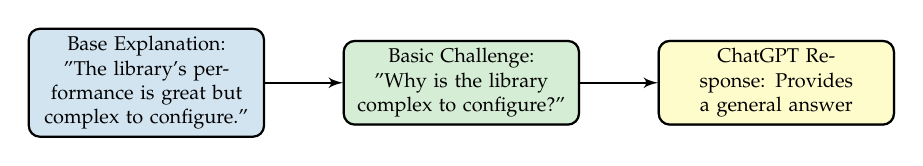
\begin{tikzpicture}[node distance=5cm, auto, thick, scale=0.8, transform shape]
      % Define styles for active and inactive nodes
      \tikzstyle{activeblock} = [rectangle, draw, text width=3.5cm, text centered, rounded corners, minimum height=1cm, font=\small, opacity=1]
      \tikzstyle{inactiveblock} = [rectangle, draw, text width=3.5cm, text centered, rounded corners, minimum height=1cm, font=\small, opacity=0.3]
      \tikzstyle{activeline} = [draw, -latex', opacity=1]
      \tikzstyle{inactiveline} = [draw, -latex', opacity=0.3]
    
      % Nodes
      \node<1-3> [activeblock, fill=blue!20] (base) {Base Explanation: \par "The library's performance is great but complex to configure."};
      \node<1> [inactiveblock, fill=green!20, right of=base] (basic) {Basic Challenge: \par "Why is the library complex to configure?"};
      \node<1> [inactiveblock, fill=yellow!20, right of=basic] (response) {ChatGPT Response: Provides a general answer};
      
      \node<2-3> [activeblock, fill=green!20, right of=base] (basic) {Basic Challenge: \par "Why is the library complex to configure?"};
      \node<2> [inactiveblock, fill=yellow!20, right of=basic] (response) {ChatGPT Response: Provides a general answer};
      
      \node<3> [activeblock, fill=yellow!20, right of=basic] (response) {ChatGPT Response: Provides a general answer};
    
      % Arrows
      \path<1> [inactiveline] (base) -- (basic);
      \path<2-3> [activeline] (base) -- (basic);
    
      \path<1-2> [inactiveline] (basic) -- (response);
      \path<3> [activeline] (basic) -- (response);
    \end{tikzpicture}
    
    
  \end{center}
\end{frame}

% Animation: Mutation Impact (Step 2)
\begin{frame}
  \frametitle{Example of Mutation Impact - Mutation Challenge}
  \begin{itemize}
    \item \textbf{Mutation Challenge}:
    \begin{itemize}
      \item Question: "Why is the library complex to configure, especially when integrating with legacy systems?"
      \item ChatGPT Response: Reveals inconsistencies or additional issues
    \end{itemize}
  \end{itemize}
  \begin{center}
    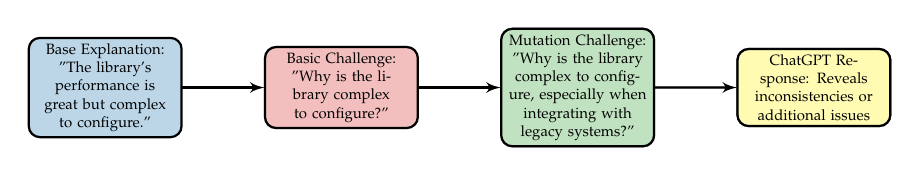
\begin{tikzpicture}[node distance=5cm, auto, thick, scale=0.6, transform shape]
      % Define styles for active and inactive nodes with different colors
      \tikzstyle{activeblock} = [rectangle, draw, text width=3cm, text centered, rounded corners, minimum height=1cm, font=\small, opacity=1]
      \tikzstyle{inactiveblock} = [rectangle, draw, text width=3cm, text centered, rounded corners, minimum height=1cm, font=\small, opacity=0.3]
      \tikzstyle{activeline} = [draw, -latex', opacity=1]
      \tikzstyle{inactiveline} = [draw, -latex', opacity=0.3]

      % Nodes with different colors for active states
      \node<1-4> [activeblock, fill=blue!30] (base) {Base Explanation: \par "The library's performance is great but complex to configure."};
      \node<1> [inactiveblock, fill=red!30, right of=base] (basic) {Basic Challenge: \par "Why is the library complex to configure?"};
      \node<1> [inactiveblock, fill=green!30, right of=basic] (mutation) {Mutation Challenge: \par "Why is the library complex to configure, especially when integrating with legacy systems?"};
      \node<1> [inactiveblock, fill=yellow!30, right of=mutation] (response) {ChatGPT Response: Reveals inconsistencies or additional issues};
      
      \node<2-4> [activeblock, fill=red!30, right of=base] (basic) {Basic Challenge: \par "Why is the library complex to configure?"};
      \node<2> [inactiveblock, fill=green!30, right of=basic] (mutation) {Mutation Challenge: \par "Why is the library complex to configure, especially when integrating with legacy systems?"};
      \node<2> [inactiveblock, fill=yellow!30, right of=mutation] (response) {ChatGPT Response: Reveals inconsistencies or additional issues};
      
      \node<3-4> [activeblock, fill=green!30, right of=basic] (mutation) {Mutation Challenge: \par "Why is the library complex to configure, especially when integrating with legacy systems?"};
      \node<3> [inactiveblock, fill=yellow!30, right of=mutation] (response) {ChatGPT Response: Reveals inconsistencies or additional issues};
      
      \node<4> [activeblock, fill=yellow!30, right of=mutation] (response) {ChatGPT Response: Reveals inconsistencies or additional issues};
      
      % Arrows
      \path<1> [inactiveline] (base) -- (basic);
      \path<2-4> [activeline] (base) -- (basic);
      
      \path<1-2> [inactiveline] (basic) -- (mutation);
      \path<3-4> [activeline] (basic) -- (mutation);
      
      \path<1-3> [inactiveline] (mutation) -- (response);
      \path<4> [activeline] (mutation) -- (response);
    \end{tikzpicture}
  \end{center}
\end{frame}


% Slide: Limitations Identified (Text)
\begin{frame}{Limitations of CID}
  \begin{itemize}
      \item \textbf{Dataset and Labeling Constraints}
      \begin{itemize}
          \item Relies on Stack Overflow data
          \item Variability and potential bias in human-annotated labels
      \end{itemize}
      
      \item \textbf{Similarity Measurement Challenges}
      \begin{itemize}
          \item Current metrics may struggle with complex or nuanced responses.
          \item Potential for misclassifications due to inadequate similarity assessments.
      \end{itemize}
      
      \item \textbf{Limited Scope and Generalizability}
      \begin{itemize}
          \item Evaluated primarily on software library selection tasks.
          \item Effectiveness on other SE tasks remains unexplored.
      \end{itemize}
  \end{itemize}
\end{frame}



% Slide: Summary of Evaluation (Text)
% \begin{frame}
%   \frametitle{Summary of Evaluation}
%   \begin{itemize}
%     \item \textbf{CID Performance}:
%     \begin{itemize}
%       \item Effectively detects incorrect responses
%       \item Mutation challenges are crucial for enhanced performance
%     \end{itemize}
%     \item \textbf{Implications}:
%     \begin{itemize}
%       \item Provides a tool for developers to assess ChatGPT's responses
%       \item Helps build trust and reliability in using AI assistants
%     \end{itemize}
%   \end{itemize}
%   \vspace{0.1cm}
%   \begin{center}
%   \begin{tikzpicture}[thick, scale=0.6, every node/.style={align=center}]
%     % Define styles for the nodes
%     \tikzstyle{block} = [circle, draw, text width=1.2cm, text centered, minimum height=1.2cm, font=\tiny, fill opacity=0.9]
    
%     % Nodes arranged on the circumference of a circle
%     \node [block, fill=blue!20] (perf) at (90:2cm) {CID\\Performance};
%     \node [block, fill=green!20] (mut) at (210:2cm) {Mutation\\Challenges};
%     \node [block, fill=yellow!20] (impl) at (330:2cm) {Implications};
    
%     % Curved arrows between nodes
%     \draw [->, thick, bend right=30] (perf) to (mut);
%     \draw [->, thick, bend right=30] (mut) to (impl);
%     \draw [->, thick, bend right=30] (impl) to (perf);
%   \end{tikzpicture}
%   \end{center}
% \end{frame}


%----------------------------------
% Conclusion Section
%----------------------------------
\section{Conclusion}

% Slide: Conclusion Overview
\begin{frame}
  \frametitle{Conclusion}
  \begin{itemize}
    \item \textbf{Recap of Research}:
    \begin{itemize}
     \only<1>{\item Explored developers' reliance on ChatGPT
      \item Identified concerns about response correctness}
      \only<2>{\item Developed CID to detect incorrect ChatGPT responses}
      \only<3>{\item Evaluted the performance of CID with relevant metrics}
    \end{itemize}
    \vspace{0.5cm}
    \begin{center}
    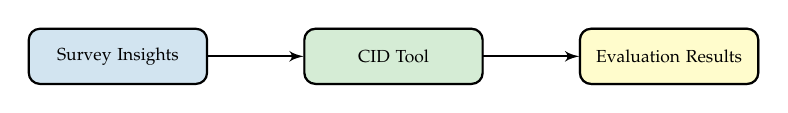
\begin{tikzpicture}[node distance=5cm, auto, thick, scale=0.7, transform shape]
      % Define styles for active and inactive nodes
      \tikzstyle{activeblock} = [rectangle, draw, text width=3cm, text centered, rounded corners, minimum height=1cm, font=\small, opacity=1]
      \tikzstyle{inactiveblock} = [rectangle, draw, text width=3cm, text centered, rounded corners, minimum height=1cm, font=\small, opacity=0.3]
      \tikzstyle{activeline} = [draw, -latex', opacity=1]
      \tikzstyle{inactiveline} = [draw, -latex', opacity=0.3]
    
      % Nodes
      \node<1-3> [activeblock, fill=blue!20] (survey) {Survey Insights};
      \node<1> [inactiveblock, fill=green!20, right of=survey] (cid) {CID Tool};
      \node<1> [inactiveblock, fill=yellow!20, right of=cid] (eval) {Evaluation Results};
    
      \node<2-3> [activeblock, fill=green!20, right of=survey] (cid) {CID Tool};
      \node<2> [inactiveblock, fill=yellow!20, right of=cid] (eval) {Evaluation Results};
    
      \node<3> [activeblock, fill=yellow!20, right of=cid] (eval) {Evaluation Results};
    
      % Arrows
      \path<1> [inactiveline] (survey) -- (cid);
      \path<2-3> [activeline] (survey) -- (cid);
    
      \path<1-2> [inactiveline] (cid) -- (eval);
      \path<3> [activeline] (cid) -- (eval);
    \end{tikzpicture}
  \end{center}
  \end{itemize}
\end{frame}


% Slide: Limitations
\begin{frame}
  \frametitle{Limitations}
  % \begin{itemize}
  %   \item \textbf{Dataset Dependence}
  %   \item \textbf{Similarity Measures}
  %   \item \textbf{Scope of Evaluation}
  % \end{itemize}
  \vspace{1cm}
  \begin{center}
    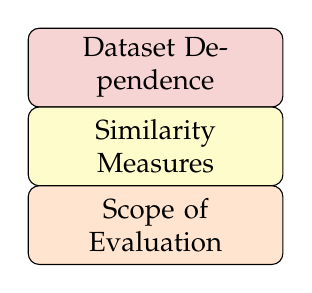
\begin{tikzpicture}
      \node [block, fill=red!20] (data) {Dataset Dependence};
      \node [block, fill=yellow!20, below of=data] (sim) {Similarity Measures};
      \node [block, fill=orange!20, below of=sim] (scope) {Scope of Evaluation};
    \end{tikzpicture}
    % \captionof{figure}{Summary of Limitations}
    
  \end{center}
  \begin{center}
  \vspace{0.5cm}
   \textbf{Summary of Limitations}
  \end{center}
\end{frame}

% Slide: Future Work
\begin{frame}
  \frametitle{Future Work}
  \begin{center}
    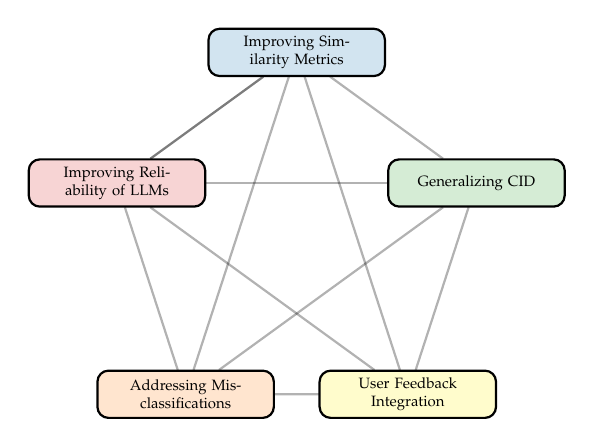
\begin{tikzpicture}[node distance=3cm, auto, thick, scale=0.6, transform shape]
      % Define node style
      \tikzstyle{block} = [rectangle, draw, rounded corners, text centered, text width=3.5cm, minimum height=1cm, font=\small]
    
      % Define pentagonal positions
      \node [block, fill=blue!20] (sim) at (90:4cm) {Improving Similarity Metrics};
      \node [block, fill=green!20] (gen) at (18:4cm) {Generalizing CID};
      \node [block, fill=yellow!20] (user) at (306:4cm) {User Feedback Integration};
      \node [block, fill=orange!20] (mis) at (234:4cm) {Addressing Misclassifications};
      \node [block, fill=red!20] (llm) at (162:4cm) {Improving Reliability of LLMs};
    
      % Undirected edges for full connectivity with reduced opacity
      \draw [-, thick, opacity=0.3] (sim) -- (gen);
      \draw [-, thick, opacity=0.3] (gen) -- (user);
      \draw [-, thick, opacity=0.3] (user) -- (mis);
      \draw [-, thick, opacity=0.3] (mis) -- (llm);
      \draw [-, thick, opacity=0.3] (llm) -- (sim);
    
      % Additional edges for full connectivity
      \draw [-, thick, opacity=0.3] (sim) -- (user);
      \draw [-, thick, opacity=0.3] (sim) -- (mis);
      \draw [-, thick, opacity=0.3] (sim) -- (llm);
    
      \draw [-, thick, opacity=0.3] (gen) -- (mis);
      \draw [-, thick, opacity=0.3] (gen) -- (llm);
    
      \draw [-, thick, opacity=0.3] (user) -- (llm);
    \end{tikzpicture}
    
    
    
    % \captionof{figure}{Future Work Roadmap}
    \vspace{0.5cm}
   \textbf{Future Work Roadmap}
  \end{center}
\end{frame}

\begin{frame}[allowframebreaks]
  \frametitle{References}
  
  \small
  \bibliographystyle{ACM-Reference-Format}
  
  \begin{thebibliography}{10}
  
  \bibitem{azaria2023internal}
  Amos Azaria and Tom Mitchell.
  \newblock The internal state of an {LLM} knows when it's lying.
  \newblock \emph{arXiv preprint arXiv:2304.13734}, 2023.
  
  \bibitem{jang2023consistency}
  Myeongjun Jang and Thomas Lukasiewicz.
  \newblock Consistency analysis of {ChatGPT}.
  \newblock \emph{arXiv preprint arXiv:2303.06273}, 2023.
  
  \bibitem{manakul2023selfcheckgpt}
  Potsawee Manakul, Adian Liusie, and Mark~J.~F. Gales.
  \newblock {SelfCheckGPT}: Zero-resource black-box hallucination detection for
    generative large language models.
  \newblock \emph{arXiv preprint arXiv:2303.08896}, 2023.
  
  \bibitem{feldman2023trapping}
  Philip Feldman, James~R. Foulds, and Shimei Pan.
  \newblock Trapping {LLM} hallucinations using tagged context prompts.
  \newblock \emph{arXiv preprint arXiv:2306.06085}, 2023.
  
  \bibitem{elazar2021measuring}
  Yanai Elazar, Nora Kassner, Shauli Ravfogel, Abhilasha Ravichander, Eduard
    Hovy, Hinrich Schütze, and Yoav Goldberg.
  \newblock Measuring and improving consistency in pretrained language models.
  \newblock \emph{Transactions of the Association for Computational Linguistics},
    9:1012--1031, 2021.
  
  \bibitem{larios2020selecting}
  Enrique Larios~Vargas, Maurício Aniche, Christoph Treude, Magiel Bruntink, and
    Georgios Gousios.
  \newblock Selecting third-party libraries: The practitioners' perspective.
  \newblock In \emph{Proceedings of the 28th ACM Joint Meeting on European
    Software Engineering Conference and Symposium on the Foundations of Software
    Engineering}, pages 245--256, 2020.
  
  \bibitem{uddin2017opiner}
  Gias Uddin and Foutse Khomh.
  \newblock {OPINER}: An opinion search and summarization engine for {APIs}.
  \newblock In \emph{Proceedings of the 32nd IEEE/ACM International Conference on
    Automated Software Engineering}, pages 978--983, 2017.
  
  \bibitem{uddin2019understanding}
  Gias Uddin, Olga Baysal, Latifa Guerrouj, and Foutse Khomh.
  \newblock Understanding how and why developers seek and analyze {API}-related
    opinions.
  \newblock \emph{IEEE Transactions on Software Engineering}, 47(4):694--735,
    2019.
  
  \bibitem{wang2020difftech}
  Han Wang, Chunyang Chen, Zhenchang Xing, and John Grundy.
  \newblock {DiffTech}: A tool for differencing similar technologies from
    question-and-answer discussions.
  \newblock In \emph{Proceedings of the 28th ACM Joint Meeting on European
    Software Engineering Conference and Symposium on the Foundations of Software
    Engineering}, pages 1576--1580, 2020.
  
  \bibitem{ribeiro2020beyond}
  Marco~Tulio Ribeiro, Tongshuang Wu, Carlos Guestrin, and Sameer Singh.
  \newblock Beyond accuracy: Behavioral testing of {NLP} models with {CheckList}.
  \newblock \emph{arXiv preprint arXiv:2005.04118}, 2020.

  \bibitem[Shen et~al\mbox{.}(2022)]%
        {shen2022natural}
  Qingchao Shen, Junjie Chen, Jie~M Zhang, Haoyu Wang, Shuang Liu, and Menghan Tian.
  \newblock Natural test generation for precise testing of question answering software. In {\emph{Proceedings of the 37th IEEE/ACM International Conference on Automated Software Engineering}}. pages 1--12.

  \vspace{0.5cm}
  \textbf{\Large Link to Orignal Paper\\}
  \href{https://dl.acm.org/doi/abs/10.1145/3597503.3639194}{ChatGPT Incorrectness Detection in Software Reviews}
  
  \end{thebibliography}
  
  \end{frame}

  

\setbeamercolor{background canvas}{bg=blue!20} % Set the background color globally for the slide
\begin{frame}
  \begin{center}
    \vspace{1cm} % Adjust vertical positioning
    {\Huge \textbf{\textit{Thank You!}}} % Large, aesthetic text
  \end{center}
\end{frame}







%------------------

\end{document}
